\documentclass[a4paper,14pt]{extarticle}
\usepackage{amsfonts} % cursed Z symbol
\usepackage{extsizes}
\usepackage{multicol}
\usepackage{amsmath}
\usepackage{float}
\usepackage{graphicx}
\usepackage{hyperref}
\usepackage{enumitem}
\usepackage{cancel}
\graphicspath{ {./images} }
\usepackage[margin=1in]{geometry}
% \usepackage{textcomp}
\title{Esercizi di Algebra}
\author{per scuole superiori}
\date{Settembre 2023}

\begin{document}

\maketitle
\tableofcontents
\newpage

\section{Introduzione}

Questa è una modesta raccolta di esercizi di matematica che ho 
compilato per aiutare i miei figli quando ne avevano bisogno.

Sono un po' in inglese e un po' in italiano perché
si tratta di materiale che ho copiato a piene mani da ogni 
sorta di risorsa trovata su internet.

L'unico mio contributo è consistito nella formattazione in  \LaTeX, cosa che ha richiesto 
dell' impegno, ragion per cui ho deciso di mettere tutto online su \href{https://github.com/davidauz}{github}\footnote{\texttt{https://github.com/davidauz}}
nel caso qualcun altro sia interessato.

Non me ne vogliano professori ed autori per essermi appropriato indebitamente dei frutti del loro lavoro.

Lo sanno tutti che i libri scolastici ed in particolare gli esercizi sono copiati da un autore 
all'altro, formando una catena di copiature che si può seguire a ritroso fino ad arrivare a 
Talete\footnote{Talete di Mileto (c. 624-546 A.C.), il ``Padre della Geometria"}.

Dove possibile ho riportato i riferimenti dei siti da dove ho copiato il materiale.

Un ringraziamento particolare a \href{https://www.risingpirates.com}{risingpirates} per avermi dato il permesso di
utilizzare materiale dal loro sito.

Detto questo, se qualcuno si dovesse sentire particolarmente violato nel trovare uno dei 
suoi esercizi in questa raccolta me lo faccia sapere e lo toglierò subito.

Allo stesso modo nel più probabile caso in cui qualcuno dovesse trovare errori, oppure avesse da 
proporre del nuovo materiale, sarò ben felice di effettuare le relative correzioni ed integrazioni.


\section{Rational Zero Theorem}\label{subsec:s_polynomials}

\subsection{Statement}

The rational zero theorem states that each rational zero(s) of a polynomial with integer coefficients 
\begin{equation}
f(x) = a_nx^n+a_{n-1}x^{n-1}+.......+a_2x^2+a_1x+a_0
\end{equation}
is of the form $\frac{p}{q}$, where
\begin{itemize}
\item $p$ is a factor of the constant $a_0$ (the one without the $x$)
\item $q$ is a factor of the leading coefficient $a_n$ (the one with the highest power of $x$)
\item $p$ and $q$ are relatively prime (i.e., the fraction $\frac{p}{q}$ is in its simplest form)

Example: 6 and 18 are not relatively prime because the fraction $\frac{6}{18}$ can be simplified to $\frac{1}{3}$
\item The integer coefficients are positive or negative integers: $a_{i}\in \mathbb{Z}$ 

This means that the theorem cannot be applied to a polynomial like $\frac{1}{3}x^3+\sqrt{2}x+3$.
\item $a_{0}$ , $a_{n}\neq 0$.
\end{itemize}

In other words

\begin{equation}
\frac{p}{q} = \frac{\textrm{factor of }a_0}{\textrm{factor of }a_n}
\end{equation}

Example:

\begin{equation}
2x^3-5x^2-4x+3=0
\end{equation}

\begin{itemize}
\item $p=\textrm{all the prime factors of 3, positive or negative:} \pm 1 \pm 3$
\item $q=\pm 1\pm 2$
\end{itemize}

\subsection{Usage}


We can use the Rational Zeros Theorem to find all the rational zeros of a polynomial. Here are the steps:
\begin{enumerate}
\item Arrange the polynomial in descending order\

(In the example: $2$, $-5$, $-4$, $3$)
\item Write down all the factors of the constant term.

These are all the possible values of $p$. ($p=\pm 1 \pm 3$)
\item Write down all the factors of the leading coefficient. 

These are all the possible values of $q$. ($q=\pm 1\pm 2$)
\item Write down all the possible values of $\pm \frac{p}{q}$.

Simplify each value and cross out any duplicates.  ( $\pm 1 \pm \frac{1}{2} \pm 3 \pm \frac{3}{2}$ )
\item Use the division algorithm to determine the values of for which $P(x) = 0$.

These are all the rational roots of $P(x)$.
\end{enumerate}


\section{Long division with polynomials}

\setcounter{equation}{0}
È un algoritmo per calcolare la divisione tra un polinomio e un altro.

% https://www.youtube.com/watch?v=_FSXJmESFmQ
\subsection{Esempio uno}

Dividere $x^2+5x+6$ (il dividendo) per $x+2$ (il divisore).

Si incomincia a scrivere così:

\begin{figure}[H]
\centering
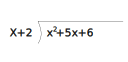
\includegraphics[width=0.8\textwidth]{polynomials.1.1.pdf}
\end{figure}

Si divide il termine più elevato del dividendo per il termine più elevato del divisore, in questo caso si divide $x^2$ per $x$.

$\frac{x^2}{x}=x$: il risultato è x, e si scrive in cima:

\begin{figure}[H]
\centering
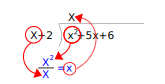
\includegraphics[width=0.8\textwidth]{polynomials.1.2.pdf}
\end{figure}

Ora moltiplico questo risultato ($x$) per il divisore ($x-2$):

\begin{equation}
(x+2)x=x^2+2x = x^2+x+0
\end{equation}

Notare che ho aggiunto $+0$ alla fine.

Ora faccio una sottrazione tra il dividendo ( $x^2+5x+6$ )e il risultato che ho trovato ora ($x^2+2x+0$).

Il risultato ($3x+6$) va scritto aggiungendo una riga in basso.

\begin{figure}[H]
\centering
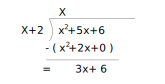
\includegraphics[width=0.8\textwidth]{polynomials.1.4.pdf}
\end{figure}

\begin{minipage}{\textwidth}
Adesso faccio la stessa cosa di prima: prendo il termine con il grado più alto del $3x+6$ e cioè $3x$, e lo divido per il termine con il grado più alto del divisore ($x-2$), che è $x$.

Il risultato della divisione ($3$) va in cima, di seguito al risultato del passaggio precedente.

\begin{figure}[H]
\centering
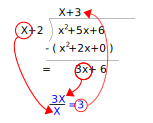
\includegraphics[width=0.8\textwidth]{polynomials.1.5.pdf}
\end{figure}
\end{minipage}

Esattamente come prima, moltiplico questo $3$ che ho trovato adesso per il divisore ($x-2$):

\begin{equation}
(x+2)3=3x+6
\end{equation}

Il risultato trovato ($3x+6$) va sottratto all'ultima riga del passaggio precedente:


\begin{figure}[H]
\centering
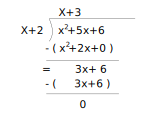
\includegraphics[width=0.8\textwidth]{polynomials.1.7.pdf}
\end{figure}

Il risultato è zero, quindi non c'è resto.

La soluzione del problema iniziale è:

\begin{equation}
\frac{x^2+5x+6}
{x+2} = x+3
\end{equation}

\begin{minipage}{\textwidth}
\subsection{Esempio due}

\setcounter{equation}{0}

\begin{equation}
\frac{2x^3+8x^2-6x+10}{x-2}
\end{equation}


\begin{figure}[H]
\centering
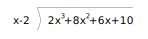
\includegraphics[width=0.8\textwidth]{polynomials.2.1.pdf}
\end{figure}

Prendo il termine di grado maggiore del dividendo ($2x^3$) e lo divido per il termine di grado maggiore del divisore ($x$).

\begin{equation}
\frac{2x^3}
{x} = 2x^2
\end{equation}

Questo $2x^2$ lo scrivo in cima come primo termine del risultato finale.

Faccio la moltiplicazione di questo primo termine ($2x^2$) per il divisore ($x-2$):

\begin{equation}
(x-2)2x^2 = 2x^3-4x^2
\end{equation}

e lo scrivo in basso aggiungendo una riga, per fare la sottrazione:

\begin{figure}[H]
\centering
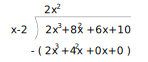
\includegraphics[width=0.8\textwidth]{polynomials.2.2.pdf}
\end{figure}

\end{minipage}

La sottrazione è questa:

\begin{equation}
2x^3+8x^2-6x+10 - (  2x^3+4x^2+0x+0 )= 12x^2-6x+10
\end{equation}

Il risultato lo scrivo sotto aggiungendo una riga.

\begin{figure}[H]
\centering
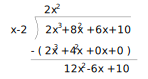
\includegraphics[width=0.8\textwidth]{polynomials.2.3.pdf}
\end{figure}

Adesso prendo il termine di grado maggiore che sta nell'ultima riga appena scritta ($12x^2$) e lo divido per il termine di grado maggiore del divisore ($x$).

\begin{equation}
\frac{12x^2}
{x} = 12x
\end{equation}

Questo $12x$ viene scritto come secondo termine del risultato finale.


\begin{figure}[H]
\centering
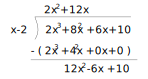
\includegraphics[width=0.8\textwidth]{polynomials.2.4.pdf}
\end{figure}

Adesso tocca alla moltiplicazione:

\begin{equation}
12x * (x-2) = 12x^2-24x
\end{equation}

Lo scrivo sotto aggiungendo una riga e faccio la sottrazione:

\begin{equation}
12x^2-6x+10-( 12x^2-24x ) = 18x+10
\end{equation}

\begin{figure}[H]
\centering
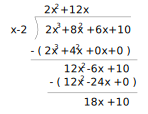
\includegraphics[width=0.8\textwidth]{polynomials.2.5.pdf}
\end{figure}

Il risultato è $18x+10$.

Il prossimo passo è la divisione 

\begin{equation}
\frac{18x}{x}=18
\end{equation}

Scrivo questo 18 come terzo termine del risultato finale, e faccio la moltiplicazione
\begin{equation}
18*(x-2) = 18x-36
\end{equation}

Aggiungo $18x-36$ come ultima riga e faccio la sottrazione.

\begin{figure}[H]
\centering
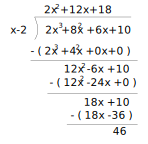
\includegraphics[width=0.8\textwidth]{polynomials.2.6.pdf}
\end{figure}

Il risultato da scrivere in fondo è 46.

Non si può più andare avanti; $\frac{46}{x-2}$ resta così, e il risultato finale dell'operazione è questo:

\begin{equation}
\frac{2x^3+8x^2-6x+10}{x-2} = 2x^2+12x+18+\frac{46}{x-2}
\end{equation}

\subsection{Esercizi}

\begin{enumerate}
\item A polynomial $P(x)=2x^3-5x^2-4x+3$ is given.
\begin{enumerate}
\item List all possible rational zeros of P
\item Find all real zeros of P
\item Sketch the graph of P
\end{enumerate}

\rightline{( Soluzione a pagina \pageref{poli_1} \label{exp_1}\label{exp_1} )}

\end{enumerate}

\newcounter{choice}
\renewcommand\thechoice{\Alph{choice}}
\newcommand\choicelabel{\thechoice.}

\newenvironment{choices}%
  {\list{\choicelabel}%
     {\usecounter{choice}\def\makelabel##1{\hss\llap{##1}}%
       \settowidth{\leftmargin}{W.\hskip\labelsep\hskip 2.5em}%
       \def\choice{%
         \item
       } % choice
       \labelwidth\leftmargin\advance\labelwidth-\labelsep
       \topsep=0pt
       \partopsep=0pt
     }%
  }%
  {\endlist}

\newenvironment{oneparchoices}%
  {%
    \setcounter{choice}{0}%
    \def\choice{%
      \refstepcounter{choice}%
      \ifnum\value{choice}>1\relax
        \penalty -50\hskip 1em plus 1em\relax
      \fi
      \choicelabel
      \nobreak\enskip
    }% choice
    % If we're continuing the paragraph containing the question,
    % then leave a bit of space before the first choice:
    \ifvmode\else\enskip\fi
    \ignorespaces
  }%
  {}

\section{Aritmetica}\label{sec:aritmetica}

\begin{enumerate}
\item \label{ari_01}

La somma

\begin{equation*}
2^{15} + 2^{15}
\end{equation*}

è uguale a

\begin{itemize}
\item[A] $2^{30}$
\item[B] $2^{16}$
\item[C] $4^{15}$
\item[D] un numero irrazionale
\item[E] $4^{30}$
\end{itemize}

( Soluzione a pagina \pageref{aris_01} )


\vspace{1cm}
\hrule
\vspace{1cm}

\item \label{ari_02}
Quanti tra i seguenti sono numeri primi?

\begin{equation*}
91,  100,  231,  440,  1003
\end{equation*}


\begin{itemize}
\item[A] Nessuno di quelli elencati
\item[B] Uno
\item[C] Due
\item[D] Tre
\item[E] Quattro
\end{itemize}


( Soluzione a pagina \pageref{aris_02} )

\item 
Nel sistema di numerazione ternaria (in base $3$) le tre sole cifre usate sono 0, 1 e 2.
Quindi, ad esempio, si hanno le uguaglianze seguenti (nelle quali il numero in basso ricorda la base):
\begin{equation*}
0_{10} = 0_3 , 1_{10} = 1_3 , 2_{10} = 2_3 ,  3_{10} = 10_3 ,  4_{10} = 11_3 , 5_{10} = 12_3
\end{equation*}

Per ulteriore chiarezza, l'ultima delle uguaglianze

\begin{equation*}
5_{10} = 12_3
\end{equation*}

si legge: ``$5$ in base $10$ è uguale a $12$ in base $3$".

Quale dei seguenti numeri è $912_{10}$ in forma ternaria?

\begin{itemize}
\item[A] 
$12101_3$
\item[B]
$20121_3$
\item[C]
$1020210_3$
\item[D]
$210212_3$
\item[E]
$1010101_3$
\end{itemize}



\end{enumerate}


\section{Logaritmi}

\subsection{links}

\href{https://www.examsolutions.net/tutorials/exam-questions-logarithms/}{examsolutions.net}\footnote{\texttt{https://www.examsolutions.net/tutorials/exam-questions-logarithms/}}
, \href{https://www.studocu.com/it/document/liceo-scientifico-vito-volterra-fabriano-ancona/chimica-dei-materiali/3-log-l10-logaritmi/45324577}{studocu.com} \footnote{\texttt{https://www.studocu.com/it/document/liceo-scientifico-vito-volterra-fabriano-ancona} 

\texttt{/chimica-dei-materiali/3-log-l10-logaritmi/45324577}}
, \href{https://assets.cambridge.org/97811076/53153/excerpt/9781107653153\_excerpt.pdf}{cambridge.org}\footnote{\texttt{https://assets.cambridge.org/97811076/53153/excerpt/9781107653153\_excerpt.pdf}}
, \href{https://www.physicsandmathstutor.com/pdf-pages/?pdf=https\%3A\%2F\%2Fpmt.physicsandmathstutor.com\%2Fdownload\%2FMaths\%2FA-level\%2FC3\%2FSolutionbank-Edexcel\%2FChapter-5\%2FP3\%2520Exercise\%25205C.pdf}{physicsandmathstutor.com}\footnote{\texttt{https://www.physicsandmathstutor.com/pdf-pages/?pdf=https\%3A\%2F\%2Fpmt.}

\texttt{physicsandmathstutor.com\%2Fdownload\%2FMaths\%2FA-level\%2FC3\%2FSolutionbank-}

\texttt{Edexcel\%2FChapter-5\%2FP3\%2520Exercise\%25205C.pdf}}


\subsection{Definizione}

Il logaritmo è la funzione inversa dell'elevamento a potenza.

\textbf{Definizione di logaritmo}:

\[
\begin{split}
\log_a(b)&=x \\
\Rightarrow
a^x&=b
\end{split}
\]

Per tutti gli $x$, $y$ e $a$ $ \in \mathbb{R}, x>0$ e $a \neq 1$:

Esempio:

\[
\begin{split}
\log_2(8)&=3 \\
\\
\Rightarrow 2^3&=8
\end{split}
\]

Il grafico del logaritmo con base maggiore di 1 cresce sempre:

\begin{figure}[H]
\centering
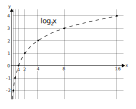
\includegraphics[width=0.7\textwidth]{log2x.pdf}
\end{figure}

Il grafico di $\log_2x$ attraversa l'asse $x$ a $x = 1$ e passa per i punti $(2, 1)$, $(4, 2)$, e $(8, 3)$

La curva si avvicina arbitrariamente all'asse $y$  senza toccarlo mai.

Per le basi minori di 1, il grafico decresce sempre:

\begin{figure}[H]
\centering
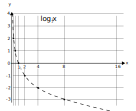
\includegraphics[width=0.7\textwidth]{log12x.pdf}
\end{figure}



\subsection{Ripassino formule sulle potenze}

\begin{enumerate}
\item $a^m \cdot a^n = a^{m+n}$
\item $\frac{a^m}{a^n}=a^{m-n}$
\item $(a^m)^n=a^{m\cdot n}$
\item $a^\frac{m}{n}=\sqrt[n]{a^m}$
\item $a^{-n}=\frac{1}{a^n}$
\item $a^n \cdot b^m=(ab)^n$
\item $\frac{a^n}{b^n}=\left(\frac{a}{b}\right)^n$
\end{enumerate}


\subsection{Relazioni e proprietà dei logaritmi}

\begin{minipage}{\textwidth}
\begin{enumerate}

\item Prodotto $\Leftrightarrow$ somma:
\[
\log_a(x\cdot y)=log_a(x) + log_a(y)
\]

\item Quoziente $\Leftrightarrow$ differenza:
\[
\log_a\left(\frac{x}{y}\right)=log_a(x) - log_a(y)
\]

\item Potenza:
\[
\log_a\left(x^y\right)=y \cdot log_a(x)
\]

\item Radice:
\[
\log_a\left(\sqrt[p]{x}\right)=\frac{log_ax}{p}
\]

\item Cambiamento di base:
\[
\log_ax=\frac{log_kx}{log_ka}\textrm{ per qualsiasi }k
\]


\item 
\[
\log_a1=0\textrm{ per tutti gli }a>0\textrm{ e }a\neq 1
\]



\item 
\[
\log_aa=1\textrm{ per tutti gli }a>0\textrm{ e }a\neq 1
\]


\item 
\[
a^{\log_ab}=b
\]


\end{enumerate}

\end{minipage}

\subsection{Cosa \textbf{NON} si può fare con i logaritmi}

\begin{enumerate}
\item $\log(x + y)$ rimane così; \textbf{NON} si può semplificare in $log x + log y$
\item $\log(e^x+e^y)$ rimane così;\textbf{NON} non si può semplificare in $x + y$
\item $(\log(x))^2$ \textbf{NON} è $2\log(x)$; la formula giusta è $\log(x^2)=2\log(x)$
\item $a^{2+\log(x)}=a^2a^{log(x)}$ \textbf{NON} $a^2+x$
\end{enumerate}

\subsection{Esercizi}
\subsubsection{Valori numerici}\label{subsec:val_num}

\begin{enumerate} % ese_numeri
\item  
\[
2\log_{12}3+4\log_{12}2=\ldots
\]
\rightline{( Soluzione a pagina \pageref{soln_1} \label{exn_1}\label{exn_1} )}


\item \[
\log_825+\log_810-3\log_85=\ldots
\]

\item \[
2\log_{10}20-(\log_{10}5+\log_{10}8)=\ldots
\]

\item \[
4\log_32-\log_34-2\log_3\sqrt{3}-\log_312=\ldots
\]

\item \[
4\cdot\log_2\left(\frac{1}{4}\right)-3\cdot\log_{\frac{1}{2}}(32)=\ldots
\]

\item\[
\frac{1}{2}\log_{\frac{2}{3}}\left(\frac{4}{9}\right)
-2\log\frac{2}{3}\left(\frac{9}{4}\right)=\ldots
\]

\end{enumerate} % ese_numeri

\subsubsection{Equazioni}\label{subsec:equazioni}

\begin{enumerate}[label={Esercizio \arabic* },wide = 1cm, font =\bfseries]

\item 
\[
\log_2\left(\frac{5}{4}x-1\right)=-2
\]
\rightline{( Soluzione a pagina \pageref{sol_1} \label{ex_1}\label{ex_1} )}

\item 
\[
\log_2\frac{2x}{x+3}=-1
\]
\rightline{( Soluzione a pagina \pageref{sol_2}\label{ex_2} )}

\item 
\[
\log_2(w^2+4w+3)=4+\log_2(w^2+w)
\]
\rightline{( Soluzione a pagina \pageref{sol_3} \label{ex_3}\label{ex_3} )}

\item \[
\log_38-3\cdot\log_3t=3
\]

\item \[
2\log_3 x-log_3(x-2)=2
\]


\item Sapendo che \[
y=3\cdot x^2
\]

verificare che \[
\log_3 y = 1 + 2\log_3 x
\]

\item \[
1+2\log_3 x = \log_3 (28x -9)
\]


\item \[
5^{(2x)}-12\cdot 5^x + 35 = 0
\]

\item \[
7^{2x}-4\cdot 7^x+3=0
\]


\item\[
\frac{
\log_232+\log_216
}{
\log_2x
}=\log_2x
\]

\item Sapendo che $a$ e $b$ sono positivi, risolvere

\[
\left\{
\begin{array}{ll}
a = 3b\\
\log_3 a + \log_3 b = 2
\end{array}
\right.
\]


\item \[
\log_2(11-6x) = 2\cdot \log_2(x-1)+3
\]

\item \[
2\log_2(x+15)-\log_2x=6
\]



\end{enumerate}


\subsubsection{Multiple Choice}\label{subsec:mult_choice}

Soluzioni a pagina \pageref{sol_mc} \label{ex_mc}\label{ex_mc}

\begin{enumerate}

\item Per $a>0$ e $a\neq 1$ quale delle seguenti affermazioni è corretta?

\begin{choices}
\choice Se $M=N$ allora $\log_aM=\log_aN$
\choice Se $\log_aM=\log_aN$ allora $M=N$
\choice Se $\log_aM^2=\log_aN^2$ allora $M=N$
\choice Se $M=N$ allora $\log_aM^2=\log_aN^2$
\end{choices}

\item Se $\log_ab=c$, allora \ldots

\begin{choices}
\choice $a^c=b$
\choice $a^b=c$
\choice $c^a-b$
\choice $c^b=a$
\end{choices}

\item Il dominio del numero reale $a$ nella formula $b=\log_{a-2}(5-a)$ è \ldots

\begin{choices}
\choice $(-\infty, 5)$
\choice $(2, 5)$
\choice $(2, 3)\cup(3, 5)$
\choice $(2, +\infty)$
\end{choices}

\item Data l'equazione
\[
\left(\frac{1}{2}\right)^3=\frac{1}{8}
\]

Quale delle seguenti affermazioni è corretta?


\begin{choices}
\choice $\log_{\frac{1}{2}}3=\frac{1}{8}$
\choice $\log_{\frac{1}{2}}\frac{1}{8}=3$
\choice $\log_{\frac{1}{8}}\frac{1}{2}=3$
\choice $\log_3\frac{1}{2}=\frac{1}{8}$
\end{choices}

\item Qual'è il valore della seguente espressione?

\[
3^{2+\frac{1}{2}\log_32}
\]

\begin{choices}
\choice $9+\sqrt{2}$
\choice $9+\frac{\sqrt{2}}{2}$
\choice $9\sqrt{2}$
\choice $10$
\end{choices}

\end{enumerate}

\subsubsection{Completare le espressioni date}\label{subsec:compl_espr}


\begin{enumerate}
\item \[
\log_3(2x-1)=1\textrm{, }x=\ldots?
\]


\item 
\[ % completare
ln(lg 10)+ \sqrt{(\pi -4)^2}=\ldots?
\]
\rightline{( Soluzione a pagina \pageref{sol_4_5} \label{ex_4_5}\label{ex_4_5} )}


\item 
Data la seguente funzione:

\[
f(3x)=\log_2{\sqrt{\frac{9x+1}{2}}}
\]

Quanto vale $f(1)$?

\rightline{( Soluzione a pagina \pageref{sol_5} \label{ex_5}\label{ex_5} )}

\end{enumerate}

\subsubsection{Domanda e risposta}\label{subsec:dom_risp}


\begin{enumerate}
\item
\[
\log_5(log_3x)=0\textrm{, }x=\ldots?
\]

\item
\[
\log_3(lg x)=1\textrm{, }x=\ldots?
\]

\item
\[
lg[\log_2(lg x)]=0\textrm{, }x=\ldots?
\]

\item

Trovare il valore di $\frac{x^2}{y}$ sapendo che 

\[
\left\{
\begin{array}{ll}
\log_\frac{1}{2} x=m\\
\log_{\frac{1}{4}}y=m+2
\end{array}
\right.
\]

\rightline{( Soluzione a pagina \pageref{sol_6} \label{ex_6}\label{ex_6} )}

\item

\[
\log_3(x+1)=3-log_3(x+7)
\]

\rightline{( Soluzione a pagina \pageref{sol_7} \label{ex_7}\label{ex_7} )}

\item

\[
\log(x^2)=(log(x))^2 
\]

\rightline{( Soluzione a pagina \pageref{sol_8} \label{ex_8}\label{ex_8} )}


\item
\[
\log(x-1)-log(x+1)=log(x-3)-log(x-2)
\]

\rightline{( Soluzione a pagina \pageref{sol_9} \label{ex_9}\label{ex_9} )}


\item Trovare $x$ per 

\[
4\cdot 5^{x+1} = 3^x
\]

\rightline{( Soluzione a pagina \pageref{sol_10} \label{ex_10}\label{ex_10} )}

\item 
\[
5^{3x+1}=15
\]

\item 
\[
3^{2x+1}=4^{x-2}
\]

\item 
\[
3\cdot 2^{x-3}=\frac{1}{5^{2x}}
\]


\item 
\[
3^{2x+1}-11\cdot 3^x=4
\]

\rightline{( Soluzione a pagina \pageref{sol_11} \label{ex_11}\label{ex_11} )}

\item
\[
2^{2x}-5 \cdot 2^x + 4 = 0
\]

\item
\[
e^x-6\cdot e^{-x}=5
\]

\item
\[
\left\{
\begin{array}{ll}
e^{x+y}=6\\
e^x+e^y=5
\end{array}
\right.
\]

\item 

Date le relazioni:

\begin{itemize}
\item $x = \log a$
\item $y = \log b$
\item $z = \log c$
\end{itemize}

Scrivere $2x+y-\frac{1}{2}z+2$ come un singolo logaritmo $\log(W)$.

\rightline{( Soluzione a pagina \pageref{sol_12} \label{ex_12}\label{ex_12} )}

\item

\[
\left\{
\begin{array}{ll}
x = \log a \\
y = \log b \\
z = \log c
\end{array}
\right.
\]

scrivere $2x + y - 0.5z + 2$ come un singolo logaritmo.

\item 

\[
\left\{
\begin{array}{ll}
a = \log x \\
b = \log y \\
c = \log z
\end{array}
\right.
\]

Trovare $a$, $b$ e $c$ per

\[
\log\left(
\frac{
10xy^2
}{
\sqrt{z}
}
\right)
\]

\item $ $

Sapendo che $\log a + 1 = \log b^2$, scrivere $a$ in termini di $b$

\item $ $

Sapendo che $\ln y = 2 + 4 \ln x$, scrivere $y$ in termini di $x$

\item $ $

Date le equazioni

\[
\left\{
\begin{array}{ll}
e^{2x}+e^y=800\\
3\ln x+\ln y = 5
\end{array}
\right.
\]

Per ognuna delle due equazioni esprimere $y$ in termini di $x$.

Dopodiché risolvere il sistema.

\item 
\[
4\log_4 x=9\log_x 4
\]
\rightline{( Soluzione a pagina \pageref{sol_13} \label{ex_13}\label{ex_13} )}

\item \[
\log_4x+\log_4(x-6)=2
\]

\item \[
2\log_2 x-\log_2(x+1)=3
\]

\item \[
25\log_2x=\log_x2
\]

\item \[
\log_4(4-x)\log_{16}(9x^2-10x+1)
\]

\end{enumerate}

\subsubsection{Applicazioni dei logaritmi in Fisica}\label{subsec:val_num}

\begin{enumerate}

\item{\ }

\begin{center}
\fbox{\begin{minipage}{0.9\textwidth}
When a cup of tea is made, its temperature is $85^\circ$C.

After 3 minutes the tea has cooled to $60^\circ$C.

That the temperature $T(^\circ C)$ of the cup of tea decays exponentially according to the function
\[
T = A + Ce^{-0.2t}
\]
, where $t$ is the time measured in minutes.

Find:\begin{itemize}
\item the values of $A$ and $C$
\item the time it takes for the tea to cool to $40^\circ$C.
\end{itemize}

\end{minipage}}
\end{center}
\rightline{( Soluzione a pagina \pageref{solf_1} \label{exf_1}\label{exf_1} )}

\item{\ }

\begin{center}
\fbox{\begin{minipage}{0.9\textwidth}
The amount of reactant, $V$ (grams), in a chemical reaction decays exponentially according to the function

\[
V = M + Ce^{-0.32t}
\]

where $t$ is the time in seconds since the start of the reaction.

Initially there was $4.5 g$ of reactant, and this had decayed to $2.6 g$ after $7$ seconds.

Find:\begin{itemize}
\item the values of $C$
\item the value that the amount of reactant approaches in the long term.
\end{itemize}

\end{minipage}}
\end{center}

\vspace{0.5cm}

\item{\ }

\begin{center}
\fbox{\begin{minipage}{0.9\textwidth}
A population of bacteria grows according to the model 

\[
P = Ae^{kt}
\]

where $P$ is the size of the population after $t$ minutes.

Given that after $2$ minutes there are $200$ bacteria and after $5$ minutes there are $1500$ bacteria, find the size of the population after 10 minutes.

\end{minipage}}
\end{center}

\end{enumerate}


\subsubsection{Problemi misti}\label{subsec:prob_mix}

\begin{enumerate}
\item Risolvere 
\[
3\cdot 9^x -10\cdot 3^x + 3 = 0
\]
\item Risolvere 
\[
2^{3x+1}=5^{5-x}
\]
\item Risolvere 
\[
\left\{
\begin{array}{ll}
\ln x^2 + \ln y =15\\
\ln x + \ln y^3 = 10
\end{array}
\right.
\]
\item Esprimere $x$ in termini di $y$:
\[
y=\ln x-\ln(x+2)+\ln(x^2-4)\\
\]
\item La curva $y=4\ln(x-a)$ passa per il punto $(5, \ln 16)$; trovare a
\item
\begin{enumerate}
\item 
An economic model predicts that the demand $D$, for a new product will grow according to the equation

\[
D = A - Ce^{-0.2t}
\]
where $t$ is the number of days since the product launch.
After 10 days the demand is 15,000 and it is increasing at a rate of 325 per day.

\begin{enumerate}
\item Find the value of $C$.
\item Find the initial demand for the product.
\item Find the long-term demand predicted by this model.
\end{enumerate}
\item  An alternative model is proposed, in which the demand grows according to the formula

\[
D=B\ln\left(
\frac{
t+10
}{
5
}
\right)
\]
The initial demand is the same as that for the first model.

\begin{enumerate}
\item Find the value of $B$.
\item What is the long-term prediction of this model?
\end{enumerate}

\item After how many days will the demand predicted by the second model become larger than the demand predicted by the first model?

\end{enumerate}
\end{enumerate}

\subsubsection{Esercizi Difficili}\label{subsec:eser_diff} %esercizi

\begin{enumerate} % esercizi difficili
\item Trovare la soluzione di % esercizi difficili
\[
2^{3x-4}\cdot3^{2x-5}=36^{x-2}
\]
scritta come $\frac{\ln p}{\ln q}$ dove $p$ e $q$ sono interi.
\item Date le espressioni % esercizi difficili
\[
\log_a b^2=c^2
\]

\[
\log_b a = c+1
\]
esprimere $a$ in termini di $b$.
\item  % esercizi difficili
In a physics experiment, the technician measured how the force $F$ exerted by a spring depends on its extension $x$.

She then plotted the values of $a = \ln F$ and $b = \ln x$ on a graph, with $b$ on the horizontal axis and $a$ on the vertical axis.

The graph was a straight line, passing through the points $(2, 4.5)$ and $(4, 7.2)$.

Find an expression for $F$ in terms of $x$.

\item Math Olympiad question!  

\[
25^x-15^x=9^x
\]
\rightline{( Soluzione a pagina \pageref{solf_2} \label{exf_2}\label{exf_2} )}


\item 

\[
100^{\left(\frac{1}{2}\lg9-lg2\right)}-\log_98\cdot\log_4\sqrt[3]{3}
\]

\rightline{( Soluzione a pagina \pageref{solf_3} \label{exf_3}\label{exf_3} )}


\end{enumerate} % esercizi difficili



\section{Trigonometria}\label{subsec:ss_trigo}

\subsection{Definizioni}

\begin{figure}[H]
\centering
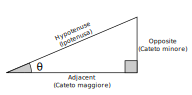
\includegraphics[width=0.7\textwidth]{trigo_01.pdf}
\end{figure}


\begin{equation}
\sin(\theta)=\frac{
\textrm{Opposite}
}{
\textrm{Hypotenuse}
}
\end{equation}

\begin{equation}
\cos(\theta)=\frac{
\textrm{Adjacent}
}{
\textrm{Hypotenuse}
}
\end{equation}

\begin{equation}
\tan(\theta)=\frac{
\textrm{Opposite}
}{
\textrm{Adjacent}
}
\end{equation}

\begin{equation}
\mathrm{cosec }(\theta)=\frac{
1
}{
\sin{\theta}
}
\end{equation}


\begin{equation}
\sec(\theta)=\frac{
1
}{
\cos{\theta}
}
\end{equation}


\begin{equation}
\cot(\theta)=\frac{
1
}{
\tan{\theta}
}
\end{equation}



\setcounter{equation}{0}

\subsection{Formule}

\begin{equation}
\cos^2\theta+\sin^2\theta=1
\end{equation}

\begin{equation}
\tan(\theta)=\frac{\sin(\theta)}{\cos(\theta)}
\end{equation}

\begin{equation}
1+\tan^2\theta=\sec^2\theta
\end{equation}

\begin{equation}
1+\cot^2\theta=\mathrm{cosec }^2\theta
\end{equation}


\begin{equation}
\sin(–\theta) = – \sin(\theta)
\end{equation}

\begin{equation}
\cos(–\theta) = -\cos(\theta)
\end{equation}

\begin{equation}
\sin(x+y)=\sin x \cos y + \cos x \sin y
\end{equation}

\begin{equation}
\sin(x-y)=\sin x \cos y - \cos x \sin y
\end{equation}


\begin{equation}
\cos(x+y)=\cos x \cos y + \sin x \sin y
\end{equation}

\begin{equation}
\cos(x-y)=\cos x \cos y - \sin x \sin y
\end{equation}




\begin{equation}
\tan(x+y)=\frac{
\tan x + \tan y
}{
1- \tan x \tan y
}
\end{equation}



\begin{equation}
\tan(x+y)=\frac{
\tan x - \tan y
}{
1 + \tan x \tan y
}
\end{equation}


\begin{equation}
\sin 2x = 2 \sin x \cos x = \frac{
2\tan x
}{
1+\tan^2x
}
\end{equation}


\begin{equation}
\cos 2x =  \cos^2 x - \sin^2 x = 
1-2\sin^2x=
2\cos^2x-1=
\frac{
1-\tan^2 x
}{
1+\tan^2x
}
\end{equation}


\begin{equation}
\tan 2x=\frac{
2\tan x
}{
1-\tan^2x
}
\end{equation}



\begin{equation}
\sin 3x=3\sin x - 4 \sin^3x
\end{equation}

\begin{equation}
\cos 3x=4\cos^3 x - 3 \cos x
\end{equation}

\begin{equation}
\tan 3x = \frac{
3\tan x - \tan^3x
}{
1-3\tan^2x
}
\end{equation}

\begin{equation}
\sin x \cos y = \frac{1}{2}[ \sin(x+y)+sin(x-y) ]
\end{equation}

\begin{equation}
\cos x + \cos y =2\cos \left(
\frac{x+y}{2}
\right)
\cos \left(
\frac{x-y}{2}
\right)
\end{equation}

\begin{equation}
\cos x - \cos y =-2\sin \left(
\frac{x+y}{2}
\right)
\sin \left(
\frac{x-y}{2}
\right)
\end{equation}


\begin{equation}
\sin x - \sin y =2\cos \left(
\frac{x+y}{2}
\right)
\sin \left(
\frac{x-y}{2}
\right)
\end{equation}

\begin{equation}
\sin x + \sin y =2\sin \left(
\frac{x+y}{2}
\right)
\cos \left(
\frac{x-y}{2}
\right)
\end{equation}

\begin{equation}
\cos\left( \frac{x}{2} \right) = \pm \sqrt{\frac{1+\cos x}{2}}
\end{equation}


\begin{equation}
\sin\left( \frac{x}{2} \right) = \pm \sqrt{\frac{1-\cos x}{2}}
\end{equation}

\setcounter{equation}{0}

\subsection{Triangoli}

\subsubsection{Links}

\href{https://www.math.it/formulario/trigonometria.htm}{math.it}\footnote{\texttt{https://www.math.it/formulario/trigonometria.htm}}
, \href{https://learning.cambridgeinternational.org/classroom/pluginfile.php/155369/mod\_resource/content/4/0580\_Teaching\_Pack\_Understanding\_Bearings\_v2.pdf}{Cambridge International}\footnote{\texttt{https://learning.cambridgeinternational.org/classroom/pluginfile.php/155369/mod\_resource/}

\texttt{content/4/0580\_Teaching\_Pack\_Understanding\_Bearings\_v2.pdf}}


\subsubsection{Teorema di Eulero}\label{subs_euler}

\begin{figure}[H]
\centering
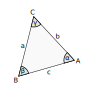
\includegraphics[width=0.3\textwidth]{trigo_04.pdf}
\end{figure}




Anche chiamato il teorema dei seni.

In un triangolo qualunque è costante il rapporto tra la misura di un lato e il seno dell’angolo opposto:


\begin{equation}
\frac{a}{\sin (\alpha)} = \frac{b}{\sin (\beta)} = \frac{c}{\sin (\gamma)}
\end{equation}

\subsubsection{Teorema delle proiezioni}

In un triangolo qualunque la misura di un lato è uguale alla somma dei prodotti delle misure di ciascuno 
degli altri due per il coseno degli angoli che essi formano con il primo:

\begin{equation}
\begin{array}{ll}
a=b\cdot \cos (\gamma) + c\cdot \cos (\beta)  \\
b=a\cdot \cos (\gamma) + c\cdot \cos (\alpha)  \\
c=a\cdot \cos (\beta) + b\cdot \cos (\alpha) 
\end{array}
\end{equation}

\subsubsection{Teorema di Carnot}\label{subs_carnot}

In un triangolo qualsiasi il quadrato di un lato è uguale alla 
somma dei quadrati degli altri due lati diminuita del doppio prodotto 
di questi due lati per il coseno dell’angolo fra essi compreso.

\begin{equation}
\begin{array}{ll}
a^2=b^2+c^2-2\cdot b\cdot c\cos(\alpha)\\
b^2=a^2+c^2-2\cdot a\cdot c\cos(\beta)\\
c^2=a^2+b^2-2\cdot a\cdot b\cos(\gamma)
\end{array}
\end{equation}

Nota: Il teorema di Carnot generalizza il Teorema di Pitagora,
a cui si riduce se si considera un triangolo rettangolo.

\subsubsection{Area di un triangolo}\label{subs_areatgl}

\begin{equation}
\textrm{Area = }\frac{1}{2}ab \sin(\gamma)
\end{equation}

\subsection{Esercizi}

\begin{enumerate} % esercizi

\item 

\begin{figure}[H]
\centering
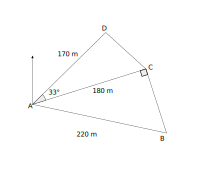
\includegraphics[width=0.7\textwidth]{trigo_02.pdf}
\end{figure}

The diagram shows five straight footpaths in a park.

\begin{itemize}
\item AB=220m
\item AC=180m
\item AD=180m
\item Angle ACB=90$^\circ$
\item Angle DAC=33$^\circ$
\end{itemize}

Calculate BC and CD.

\rightline{( Soluzione a pagina \pageref{stri_01} \label{etri_01}\label{etri_01} )}


\item 

Trovare l'altezza dell'edificio in figura in base ai dati ivi forniti.

\begin{figure}[H]
\centering
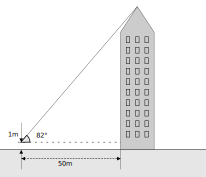
\includegraphics[width=0.7\textwidth]{trigo_05.pdf}
\end{figure}
\rightline{( Soluzione a pagina \pageref{stri_02} \label{etri_02}\label{etri_02} )}


\item 

Dimostrare che 

\[
\frac{
\cos(x)
}{
\tan(x)\cdot\left(1-\sin(x)\right)
} = 1+\frac{1}{\sin(x)}
\]
\rightline{( Soluzione a pagina \pageref{stri_03} \label{etri_03}\label{etri_03} )}

\item 

\[
\frac{
1+2\sin(x)\cos(x)
}{
\sin(x)+\cos(x)
}
=
\sin(x)+\cos(x)
\]
\rightline{( Soluzione a pagina \pageref{stri_04} \label{etri_04}\label{etri_04} )}

\item
( This item and the next 5 are from 
\href{https://www.analyzemath.com/high\textunderscore school\textunderscore math/grade\textunderscore 12/circles\textunderscore sectors\textunderscore and\textunderscore trigonometry\textunderscore problems.html}{analyzemath.com}
\footnote{\texttt{https://www.analyzemath.com/high\textunderscore school\textunderscore math/grade\textunderscore 12/circles\textunderscore sectors\textunderscore and\textunderscore}

\texttt{trigonometry\textunderscore problems.html}}
)


If the coordinates of point A, in the circle below, are (8, 0) and arc s has a length of 20 units, find the coordinates of point P in the diagram below.

\begin{figure}[H]
\centering
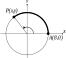
\includegraphics[width=0.5\textwidth]{analyzem01.pdf}
\end{figure}

\rightline{( Soluzione a pagina \pageref{analyzem01_s} \label{analyzem01_l})}

\end{enumerate} % esercizi



\section{Problemi vari}
\begin{enumerate}
\item 
A function $f(x)$ is defined on $\mathbb{R}$.

We have the following known items:

\begin{enumerate}
\item $f(x-1)$ is an odd function \label{laba}
\item $f(x+2)$ is an even function \label{labb}
\item In the interval $[-1,2]$, $f(x)=ax^2+b$ for some constants $a$ and $b$ \label{labc}
\item $f(1)=0$ \label{labd}
\item $f(-4)+f(3)=-3$ \label{labe}
\end{enumerate}

\vspace{1cm}
Problem: find $f(\frac{15}{2})$.

\vspace{1cm}
\hrule
\vspace{1cm}

Solution

First of all let's define the statement given at item \ref{laba}.

A function $f(x)$ is odd when $-f(x)=f(-x)$.

This does not mean that if $f(x)$ is odd, then $f(x-1)$ is odd too, or vice versa.

For example $f(x)=x^3$ is odd but $f(x)=(x-1)^3$ is not.

In this case $(x-1)$ is a function itself that we can call $g(x)=(x-1)$.

The complete statement is that $f(g(x))$ is odd:

\begin{equation}
\begin{split}
-f(g(x))&=f(g(-x))\\
\\
\textrm{with: } g(-x)&=(-x-1)\\
\\
\textrm{So: }-f(x-1)&=f(-x-1)
\end{split}
\end{equation}

The same goes for the statement at item \ref{labb}: the fact that $f(x+2)$ is even does not mean that $f(x+2)=f(-x-2)$.

Instead we must go through the same reasoning as before:

\begin{equation}
\begin{split}
f(g(x))\textrm{ is odd means that }\\
\\
f(g(x))&=f(g(-x))\\
\\
\textrm{with: } g(x)&=(x+2)\\
\\
\textrm{and: } g(-x)&=(-x+2)\\
\\
\textrm{So: }f(x+2)&=f(-x+2)
\end{split}
\end{equation}


This said, to find the solution we must first determine the $a$ and $b$ in item \ref{labc}, then find a way to convert $\frac{15}{2}$ in a way that the function $ax^2+b$ can be used in the given interval $[-1,2]$.

Since the given odd function has a big $1$ in it, let's see what happens at $x=1$.

\begin{equation}
\begin{split}
f(x) &= ax^2 + b \textrm{ in the interval [-1, 2]} \\
\\
\textrm{substituting } x &= 1 \textrm{ gives} \\
\\
f(1) = a + b &= 0 \\
\\
a+b=0\textrm{ means } b &= -a
\end{split}
\end{equation}

Next we can do the same in item \ref{labb} [that is: $f(x+2)=f(-x+2)$ ] so for $x=1$ we have

\begin{equation}
\begin{split}
f(x+2)=f(-x+2) \\
\\
f(3)=f(1)=0
\end{split}
\end{equation}

We now have values for $f(1)$ and $f(3)$, and we know that $b=-a$.

We just need another relation between $a$ and $b$ in the interval $[ -1, 2 ]$ to build a system of equations.

Item \ref{labe} tells us that $f(-4)+f(3)=-3$, so let's try using $x=3$ in item \ref{laba}:

\begin{equation}
\begin{split}
-f(x-1)&=f(-x-1) \\
\\
-f(3-1)&=f(-3-1)= \\
\\
-f(2)&=f(-4) \\
\\
\textrm{2 is in the given interval}\\
\\
\textrm{so } f(-4)=-f(2)&=-4a-b
\end{split}
\end{equation}

We now have a system of equations:

\begin{equation}
\left\{
\begin{array}{ll}
a=-b \\
-4a-b+a+b=-3
\end{array}
\right.
\end{equation}

The system gives us 

\begin{equation}
\left\{
\begin{array}{ll}
a=1 \\
b=-1
\end{array}
\right.
\end{equation}

We can now write 

\begin{equation}
\label{equa}
f(x)=x^2-1
\end{equation}

The only issue is that $\frac{15}{2}$ is not in the given interval; we can however use items \ref{laba} and \ref{labb} to find an equivalent value.

From item \ref{labb} we can write: 

\begin{equation}
\begin{split}
f\left(\frac{15}{2}\right)=f\left(\frac{11}{2}+2\right)=f\left(-\frac{11}{2}+2\right)=f\left(-\frac{7}{2}\right)
\end{split}
\end{equation}

$-\frac{7}{2}$ is still not in the given interval; let's try with item \ref{laba}:

\begin{equation}
\begin{split}
f\left(-\frac{7}{2}\right)=f\left(\frac{5}{2}-1\right)=-f\left(\frac{5}{2}-1\right)=-f\left(\frac{3}{2}\right)
\end{split}
\end{equation}

Now we can use equation \ref{equa}:

\begin{equation}
\begin{split}
f(x)&=x^2-1 \\
\\
\Rightarrow -f\left(\frac{3}{2}\right)&=-\left[ \left(\frac{3}{2}\right)^2-1\right]\\
\\
&=-\left(\frac{9}{4}-1\right) \\
\\
&=-\frac{5}{4}
\end{split}
\end{equation}

\end{enumerate}

\subsubsection{Additional exercises}\label{subsec:additional_log}

\begin{enumerate}
\item  
\begin{equation*}
2\cdot \ln(6x - 2) = 5
\end{equation*}
\rightline{ (Soluzione a pagina \pageref{sola_1}\label{exa_1} )}

\item 
\begin{equation*}
e^{4x} - 3e^{2x} + 2 = 0
\end{equation*}
\rightline{( Soluzione a pagina \pageref{sola_2}\label{exa_2} )}

\item 
\begin{equation*}
3^xe^{4x-1} = 5
\end{equation*}
\rightline{( Soluzione a pagina \pageref{sola_3}\label{exa_3} )}

\item 
% https://www.physicsandmathstutor.com/pdf-pages/?pdf=https%3A%2F%2Fpmt.physicsandmathstutor.com%2F%2Fdownload%2FMaths%2FA-level%2FPure%2FExponentials-and-Logarithms-1%2FSolomon%2F6a.%2520Mixed%2520exam-style%2520questions%2520on%2520exponentials%2520and%2520logarithms.pdf
% and
% https://www.physicsandmathstutor.com/pdf-pages/?pdf=https%3A%2F%2Fpmt.physicsandmathstutor.com%2F%2Fdownload%2FMaths%2FA-level%2FPure%2FExponentials-and-Logarithms-1%2FSolomon%2F6b.%2520Mixed%2520exam-style%2520questions%2520on%2520exponentials%2520and%2520logarithms%2520-%2520Answers.pdf

An initial investment of \$1000 is placed into a savings account that offers 2.2\% interest
every 3 months. 

The amount of money in the account, \$P, at the end of $t$ years is given by 

\begin{equation*}
P = 1000 \cdot 1.0224t
\end{equation*}

Find, to the nearest year, how long it will take for the investment to double in value. 

\rightline{( Soluzione a pagina \pageref{sola_4}\label{exa_4} )}

\end{enumerate}

\pagebreak


\section{Calcolo combinatorio}\label{subsec:calcolo_combinatorio}

\subsection{Formule}
\setcounter{equation}{0}

\begin{enumerate}

\item 
Coefficiente binomiale (binomial coefficient)

\begin{equation}
\binom{n}{k} = \frac{
n\times (n-1)\times\cdots\times(n-k+1)
}{
k\times(k-1)\times\cdots\times1
}
=\frac{n!}{k!(n-k)!}
\end{equation}



per $n,k\in \mathbb{N} ,0\leq k\leq n$

L'espressione $\tbinom{n}{k}$ si legge ``\emph{n su k}", in inglese ``\emph{n choose k}" perché ci sono $\tbinom {n}{k}$ modi di scegliere un sottoinsieme non ordinato di $k$ elementi da un insieme di $n$ elementi. 

\item
Binomial formula (o binomial identity):

\begin{equation*}
(x+y)^n=
\binom{n}{0}x^{n}y^0+
\binom{n}{1}x^{n-1}y^1+
\binom{n}{2}x^{n-2}y^2+\cdots+
\binom{n}{n-1}x^{1}y^{n-1}+
\binom{n}{n}x^{0}y^{n}
\end{equation*}

La stessa formula usando la sommatoria:

\begin{equation}
(x+y)^n=\sum_{k=0}^{n}{\binom{n}{k}x^{k}y^{n-k}}
=\sum_{k=0}^{n}{\binom{n}{k}x^{n-k}y^{k}}
\end{equation}


\item
Formula di Pascal (regola di Pascal)

\begin{equation}\label{formula_pascal}
{n \choose k}={n-1 \choose k}+{n-1 \choose k-1}
\end{equation}

\end{enumerate}

\subsection{Esercizi}

\begin{enumerate}
\item

Trovare le soluzioni di

\begin{equation*}
\binom{n}{8}=\binom{n}{6} \hspace{2cm} n \geq 8
\end{equation*}
( Soluzione a pagina \pageref{combs_01} \label{combl_01} )



\item 

\begin{equation*}
\frac{n!}{(n-3)!} = 210
\end{equation*}

( Soluzione a pagina \pageref{combs_02} \label{combl_02} )

\item
Dimostrare che 

\begin{equation*}
\sum_{k=0}^{n}{\binom{n}{k}}=2^n
\end{equation*}
( Soluzione a pagina \pageref{combs_03} \label{combl_03} )
\end{enumerate}

\section{Limiti di successioni}\label{subsec:limiti:successioni}

Definizione:

Una successione di numeri reali $(a_n)_n$ converge ad un numero reale 
$l\in \mathbb{R}$ quando per qualsiasi numero reale
$\varepsilon > 0$ esiste un indice 
$n_0\in \mathbb{N}$ tale che tutti i termini della successione con indice maggiore di 
$n_0$ hanno distanza da $l$ minore di $\varepsilon$, dove la distanza è il valore assoluto
\[
\left| a_n-l \right|
\]


La stessa definizione usando il formalismo matematico diventa:

\[
\forall \varepsilon > 0  \exists n_0\in \mathbb{N} : \left|a_n-l\right| < \varepsilon
\forall n>n_0
\]

Quando l'enunciato è vero si scrive

\[
\lim_{n\to\infty}a_n = l
\]

e si legge così: 

Il limite per n tendente all'infinito di `$a$ $n$' è `$l$'

\subsection{Esercizi}

\begin{enumerate}




\item  dimostrare che  \label{lims_00}
% https://www.youmath.it/domande-a-risposte/view/3114-verifica-limite.html
\[
\lim_{n\to + \infty}\frac{n}{2n+5}=\frac{1}{2}
\]
\rightline{ (Soluzione a pagina \pageref{limss_00} )}


\item  dimostrare che  \label{lims_01}
% https://www.youmath.it/lezioni/analisi-matematica/successioni/554-definizione-limite-successione.html
\[
\lim_{n\to + \infty}\frac{n-1}{n}=1
\]
\rightline{ (Soluzione a pagina \pageref{limss_01} )} % limits.solutions.tex

% https://www.youmath.it/esercizi/es-analisi-matematica/esercizi-successioni/1796-esercizi-risolti-sulla-verifica-del-limite-di-una-successione.html


\item Calcolare \label{lims_02}
\[
\lim_{n \to +\infty}\frac{2n+1}{3n-1}
\]
\rightline{ (Soluzione a pagina \pageref{limss_02} )} % limits.solutions.tex


\end{enumerate}

\pagebreak


\section{Il Cerchio}\label{subsec:the:circle}

Ricordiamo che l'equazione per un cerchio con centro in $(h,k)$ e raggio $r>0$ è la seguente: 

\begin{equation} \label{cerchio:equazione}
(x-h)^2+(y-k)^2=r^2
\end{equation}

\subsection{Esercizi}

\begin{enumerate}

\item  \label{circ_00}
% https://math.libretexts.org/
Write an equation of the circle centered at $(8 , -10)$ with radius $8$.
\rightline{ (Soluzione a pagina \pageref{circs_00} )}

\vspace{1cm}
\hrule
\vspace{1cm}


\item  \label{circ_01}

State the center and radius of the circle graphed below and construct the equation for it.

\begin{figure}[H]
\centering
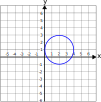
\includegraphics[width=0.6\textwidth]{circles_00.pdf}
\end{figure}


\rightline{ (Soluzione a pagina \pageref{circs_01} )}

\vspace{1cm}
\hrule
\vspace{1cm}

\item  \label{circ_02}

State the center and radius of the circle graphed below and construct the equation for it.

\begin{figure}[H]
\centering
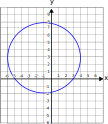
\includegraphics[width=0.6\textwidth]{circles_01.pdf}
\end{figure}


\rightline{ (Soluzione a pagina \pageref{circs_02} )}

\item  \label{circ_03}

State the center and radius of the circle described by the equation and graph it.

\begin{equation*}
\begin{split}
(a): (x-2)^2+(y+3)^2=9 \\
\\
(b): (x-2)^2+(y+5)^2=4 \\
\\
(c): (x+9)^2+y^2=25 \\
\\
(d): (x+\frac{1}{2})^2+(y-\frac{3}{5})^2=\frac{161}{100}
\end{split}
\end{equation*}


\rightline{ (Soluzione a pagina \pageref{circs_03} )}

\vspace{1cm}
\hrule
\vspace{1cm}


\item  \label{circ_04}

Find the center and radius of the circle 
\begin{equation*}
x^2+y^2-6x+8y+24=0 
\end{equation*}



\rightline{ (Soluzione a pagina \pageref{circs_04} )}

\vspace{1cm}
\hrule
\vspace{1cm}



\item  \label{geop_01}
% from savemyexams.com
A circle has equation 

\begin{equation*}
x^2+y^2+14x-6y=-41
\end{equation*}

The lines $l_1$ and $l_2$ are both tangents to the circle, 
and they intersect at the point $(0,14)$.

\begin{figure}[h]
\centering
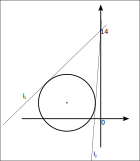
\includegraphics[width=0.4\textwidth]{01.pdf}
\end{figure}

Find the equatons of $l_1$ and $l_2$ giving your answers in the form $y=mx+c$.

( Soluzione a pagina \pageref{geos_01} )
% soluzione da qui: https://www.quora.com/A-circle-has-the-equation-x-2-6x-2y-y-2-7-The-lines-l1-and-l2-are-tangents-to-the-circle-they-intersect-at-R-0-6-How-do-you-find-the-equations-of-l1-and-l2


\vspace{1cm}
\hrule
\vspace{1cm}


\item  \label{circ_06}

Date le due circonferenze definite dalle seguenti equazioni:

\begin{equation*}
\begin{split}
(a): x^2+y^2-2x-4y-4=0 \\
\\
(b): x^2+y^2-4x-2y+4=0
\end{split}
\end{equation*}

Possiamo affermare che le due circonferenze:

\begin{itemize}
\item[A)] sono tangenti
\item[B)] sono disgiunte e la seconda è interna alla prima
\item[C)] si intersecano in due punti distinti
\item[D)] si intersecano in quattro punti distinti
\item[E)] sono disgiunte e la prima è interna alla seconda
\end{itemize}


\rightline{ (Soluzione a pagina \pageref{circs_06} )}

\vspace{1cm}
\hrule
\vspace{1cm}


%\item  \label{circ_07}
%\rightline{ (Soluzione a pagina \pageref{circs_07} )}
%
%\vspace{1cm}
%\hrule
%\vspace{1cm}
%
%
%\item  \label{circ_08}
%\rightline{ (Soluzione a pagina \pageref{circs_08} )}
%
%\vspace{1cm}
%\hrule
%\vspace{1cm}
%
%
%\item  \label{circ_09}
%\rightline{ (Soluzione a pagina \pageref{circs_09} )}
%
%\vspace{1cm}
%\hrule
%\vspace{1cm}
%
%
%\item  \label{circ_10}
%\rightline{ (Soluzione a pagina \pageref{circs_10} )}
%
%\vspace{1cm}
%\hrule
%\vspace{1cm}
%
%


\end{enumerate}

\pagebreak


\section{Funzioni} \label{sec:funzioni}

\subsection{links}


\href{https://pastpapers.papacambridge.com}{papacambridge.com}\footnote{\texttt{https://pastpapers.papacambridge.com}}


\subsection{Esercizi}

\begin{enumerate}
\item  
The function $f$ is defined for $x \in \mathbb{R}$
by 
\[
f(x) = x^2 - 6x + k
\]

where $k$ is a constant.

It is given that $f(x) > 2$ for all values of $x$.

Find the set of possible values of $k$.

\rightline{( Soluzione a pagina \pageref{solf_1} \label{exf_1} )}



\item
The equation of a line is \[ y = mx + c \] where $m$ and $c$ are constants.

The equation of a curve is \[ xy = 16 \]

\begin{enumerate}
\item Given that the line is a tangent to the curve, express $m$ in terms of $c$.
\item Given instead that $m = -4$, find the set of values of $c$ for which the line 
intersects the curve at two distinct points.
\end{enumerate}

\rightline{( Soluzione a pagina \pageref{solf_2} \label{exf_2} )}

\item
The equation of a curve is \[ y=2x^2 + kx + k - 1 \] where $k$ is a constant.

\begin{enumerate}
\item Given that the line $y=2x+3$ is tangent to the curve, find the value of $k$.
\item It is now given that $k=2$.  Express the equation of the curve in the form $y=2(x+a)^2+b$
where $a$ and $b$ are constants, and hence state the coordinates of the vertex of the curve.
\end{enumerate}

\rightline{( Soluzione a pagina \pageref{solf_3} \label{exf_3} )}

\end{enumerate}



\section{Soluzioni}

\subsection{Soluzioni di esercizi nella sezione ``\textbf{\nameref{subsec:s_polynomials}}".}

Soluzione dell'esercizio \ref{exp_1} a pagina \pageref{exp_1}\label{poli_1}


\begin{enumerate}
\item List all possible rational zeros of P.

I possibili zeri si trovano usando il \emph{Rational Zero Theorem} :

\begin{enumerate}
\item $p=\pm 1, \pm 3$
\item $q=\pm 1, \pm 2$
\item i possibili valori di $\pm \frac{p}{q}$ sono $\pm 1, \pm \frac{1}{2}, \pm 3, \pm \frac{3}{2}$
\end{enumerate}

\item Find all real zeros of P,

\begin{enumerate}
\item Sostituisco i vari valori di $\pm \frac{p}{q}$:
\setcounter{equation}{0}

\begin{itemize}

\item Provo con $1$:

\begin{equation*}
P(1)=2-5-4+3=-4
\end{equation*}

\item Provo con $-1$:

\begin{equation*}
P(-1)=-2-5+4+3=0 \Leftarrow \textrm{ trovato il primo}
\end{equation*}

\item Provo con $\frac{1}{2}$:

\begin{equation*}
\begin{split}
P\left(\frac{1}{2}\right)&=2\left(\frac{1}{2}\right)^3-5\left(\frac{1}{2}\right)^2-4\left(\frac{1}{2}\right)+3= \\
\\
\frac{2}{8}-\frac{5}{4}-\frac{4}{2}+3&=\frac{2-10-16+24}{8}=0 \Leftarrow \textrm{ trovato il secondo}
\end{split}
\end{equation*}

\item Provo con $-\frac{1}{2}$:

\begin{equation*}
\begin{split}
P\left(-\frac{1}{2}\right)=2\left(-\frac{1}{2}\right)^3&-5\left(-\frac{1}{2}\right)^2-4\left(-\frac{1}{2}\right)+3=\\
\\
-\frac{2}{8}-\frac{5}{4}+\frac{4}{2}+3&=\frac{-2-10+16+24}{8}=\\
\\
\frac{28}{8}&=3.5
\end{split}
\end{equation*}

\item Provo con $3$:

\begin{equation}
\begin{split}
P(3)=2*27-5*9-4*3+3=\\
\\
54-45-12+3=0 \Leftarrow \textrm{ trovato il terzo}
\end{split}
\end{equation}

\end{itemize}



\item Sketch the graph of P.

So che il grafico passa per i punti: $(0,-1)$, $(0, \frac{1}{2})$ e $(0, 3)$.

Calcolo $P(0)=3$ e segno anche quello.

\begin{figure}[H]
\centering
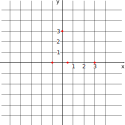
\includegraphics[width=0.5\textwidth]{function.1.pdf}
\end{figure}

Sapendo più o meno la forma delle funzioni di terzo grado posso tracciare questa curva:

\begin{figure}[H]
\centering
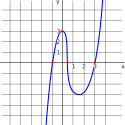
\includegraphics[width=0.5\textwidth]{function.2.pdf}
\end{figure}




\end{enumerate}

Ho trovato tre zeri: $-1$, $\frac{1}{2}$ e $3$.

Non occorre provare gli altri perché una equazione di terzo grado ha al massimo tre zeri.



\item

\end{enumerate}

\subsection{Soluzioni di esercizi nella sezione ``\textbf{\nameref{subsec:val_num}}".}

Soluzione dell'esercizio \ref{exn_1} a pagina \pageref{exn_1}\label{soln_1}
\begin{equation*}
2\log_{12}3+4\log_{12}2=\ldots
\end{equation*}

\begin{equation*}
=\log_{12}3^2+\log_{12}2^4=\log_{12}9+\log_{12}16
\end{equation*}

\begin{equation*}
=\log_{12}144=\log_{12}12^2=2\log_{12}12=2\cdot 1=2
\end{equation*}

\vspace{1cm}
\hrule
\vspace{1cm}

\subsection{Soluzioni di esercizi nella sezione ``\textbf{\nameref{subsec:equazioni}}".}

Soluzione dell' \ref{ex_1} a pagina \pageref{ex_1}\label{sol_1}

\begin{equation*}
\log_2\left(\frac{5}{4}x-1\right)=-2
\end{equation*}

Le equazioni con i logaritmi si risolvono quando tutti i termini sono dei logaritmi.

Quindi bisogna trovare il modo di trasformare tutto ciò che non lo è in un logaritmo.

In questo caso bisogna trovare un valore $a$ tale che 

\begin{equation*}
\log_2(a)=-2
\end{equation*}

cioè 

\begin{equation*}
\begin{split}
2^{-2}&=a \\
\\
\Rightarrow a&=\frac{1}{2^2} \\
\\
\Rightarrow a&=\frac{1}{4} \\
\end{split}
\end{equation*}

A questo punto il problema diventa

\begin{equation*}
\begin{split}
\log_2\left(\frac{5}{4}x-1\right)&=log_2\left(\frac{1}{4}\right) \\
\\
\frac{5}{4}x-1&=\frac{1}{4} \\
\\
\frac{5}{4}x&=\frac{5}{4} \\
\\
x&=1
\end{split}
\end{equation*}

\vspace{1cm}
\hrule
\vspace{1cm}

Soluzione dell'\ref{ex_2} a pagina \pageref{ex_2}\label{sol_2}

\begin{equation*}
\log_22\frac{2x}{x+3}=-1
\end{equation*}



Come nel caso precedente, bisogna trasformare tutti i termini in logaritmi.


Primo passo: trovare $a$ tale che:

\begin{equation*}
\begin{split}
\log_2a=-1\\
\\
2^{-1}=a\\
\\
a=\frac{1}{2}
\end{split}
\end{equation*}

Ora possiamo continuare così:

\begin{equation*}
\begin{split}
\log_2\frac{2x}{x+3}&=log_2\frac{1}{2} \\
\\
\frac{2x}{x+3}&=\frac{1}{2} \\
\\
\frac{4x}{2\cdot(x+3)}&=\frac{x+3}{2\cdot(x+3)} \\
\\
4x&=x+3 \\
\\
x&=1
\end{split}
\end{equation*}


\vspace{1cm}
\hrule
\vspace{1cm}
Soluzione dell'\ref{ex_3} a pagina \pageref{ex_3}\label{sol_3}

\begin{equation*}
\log_2(w^2+4w+3)=4+\log_2(w^2+w)
\end{equation*}

\begin{equation*}
\Rightarrow\log_2(w^2+4w+3)-\log_2(w^2+w)=4
\end{equation*}

\begin{equation*}
\Rightarrow
\log_2\left(\frac{
w^2+4w+3
}{
w^2+w
}\right) = 4\log_22
\end{equation*}

\begin{equation*}
\log_2\left(\frac{
(w+1)(w+3)
}{
w(w+1)
}\right) = 4\log_22 \textrm{ ($w\neq -1$)}
\end{equation*}

\begin{equation*}
\log_2\left(\frac{w+3}{w}\right) = \log_216
\end{equation*}

\begin{equation*}
\frac{w+3}{w}=16
\end{equation*}

\begin{equation*}
w+3=16w
\end{equation*}

\begin{equation*}
w=\frac{1}{5}
\end{equation*}

\vspace{1cm}
\hrule
\vspace{1cm}


\subsection{Soluzioni di esercizi nella sezione ``\textbf{\nameref{subsec:mult_choice}}".}

Quesiti a pagina \pageref{ex_mc}
\label{sol_mc}

\begin{enumerate}
\item A, B, D
\item A
\item C
\end{enumerate}

\vspace{1cm}
\hrule
\vspace{1cm}

Soluzione dell'esercizio \ref{ex_4_5} a pagina \pageref{ex_4_5}\label{sol_4_5}

\begin{equation*} % completare
ln(lg 10)+ \sqrt{(\pi -4)^2}=\ldots?
\end{equation*}


\begin{equation*}
ln(lg 10)+ \sqrt{(\pi -4)^2}=\ldots
\end{equation*}

\begin{equation*}
\ln(log_{10} 10) +(4-\pi)=
\end{equation*}

\begin{equation*}
\ln1+4-\pi=
\end{equation*}

\begin{equation*}
4-\pi
\end{equation*}





\vspace{1cm}
\hrule
\vspace{1cm}






Soluzione dell'esercizio \ref{ex_5} a pagina \pageref{ex_5}\label{sol_5}

Data la seguente funzione:

\begin{equation*}
f(3x)=\log_2{\sqrt{\frac{9x+1}{2}}}
\end{equation*}

Quanto vale $f(1)$?


Questa è una funzione composta:

\begin{equation*}
f(g(x)) \textrm{ con } g(x)=3x
\end{equation*}

O se preferiamo $y=3x$

Quindi 

\begin{equation*}
x=\frac{y}{3}
\end{equation*}

\begin{equation*}
f(y)=\log_2{\sqrt{\frac{9\frac{y}{3}+1}{2}}}
\end{equation*}

Ora basta sostituire $y$ con $1$

\begin{equation*}
f(1)=\log_2{\sqrt{\frac{9\frac{1}{3}+1}{2}}}
\end{equation*}



\vspace{1cm}
\hrule
\vspace{1cm}
Soluzione dell'esercizio \ref{ex_6} a pagina \pageref{ex_6}\label{sol_6}

Trovare il valore di $\frac{x^2}{y}$ sapendo che 

\begin{equation*}
\begin{split}
\log_{\frac{1}{2}}x=m \\
\\
\log_{\frac{1}{4}}y=m+2
\end{split}
\end{equation*}

\vspace{1cm}
\hrule
\vspace{1cm}

Soluzione

Uso la formula del il cambiamento di base

\begin{equation*}
\log_{\frac{1}{4}}y=\frac{
\log_{\frac{1}{2}}y
}{
\log_{\frac{1}{2}}\frac{1}{4}
}=m+2
\end{equation*}

ma $\log_{\frac{1}{2}}\frac{1}{4}$ fa 2, quindi

\begin{equation*}
\log_\frac{1}{2}y=2(m+2)
\end{equation*}

Ora posso cambiare i logaritmi in potenze:

\begin{equation*}
\begin{split}
\frac{1}{2}^m=x \\
\\
\frac{1}{2}^{2m+2}=y
\end{split}
\end{equation*}

\begin{equation*}
\frac{x^2}{y}=
\frac{
\left( \left( \frac{1}{2} \right)^m \right)^2
}{
\left( \frac{1}{2} \right) ^{(2m+2)}
}
\end{equation*}

\begin{equation*}
\frac{
\left( \frac{1}{2} \right)^{2m}
}{
\left( \frac{1}{2} \right) ^{2m} \cdot
\frac{1}{2}^2
}=4
\end{equation*}

\vspace{1cm}
\hrule
\vspace{1cm}



Soluzione dell'esercizio \ref{ex_7} a pagina \pageref{ex_7}\label{sol_7}

\begin{equation*}
\log_3(x+1)=3-log_3(x+7)
\end{equation*}

Soluzione

\begin{equation*}
\log_3(x+1)+log_3(x+7)=3
\end{equation*}

\begin{equation*}
\log_3[(x+1) \cdot (x+7)]=3
\end{equation*}

\begin{equation*}
3^3=(x+1) \cdot (x+7)
\end{equation*}



\vspace{1cm}
\hrule
\vspace{1cm}


\begin{minipage}{\textwidth}
Soluzione dell'esercizio \ref{ex_8} a pagina \pageref{ex_8}\label{sol_8}

\begin{equation*}
\log(x^2)=(log(x))^2 
\end{equation*}

Soluzione

\begin{equation*}
2\cdot \log(x)=(log(x))^2 
\end{equation*}

\begin{equation*}
\log(x)\cdot (log(x)-2)-0
\end{equation*}

Ci sono due risultati:

\begin{equation*}
\log(x)=0\textrm{ ma anche }log(x)=2
\end{equation*}

In forma di potenza abbiamo

\begin{equation*}
10^0=x \textrm{ , } 10^2=x
\end{equation*}

Le soluzioni sono quindi

\begin{equation*}
x_1=1 \textrm{ , } x_2=100
\end{equation*}

\end{minipage}



\vspace{1cm}
\hrule
\vspace{1cm}

Soluzione dell'esercizio \ref{ex_9} a pagina \pageref{ex_9}\label{sol_9}

\begin{equation*}
\log(x-1)-log(x+1)=log(x-3)-log(x-2)
\end{equation*}

\begin{equation*}
\log\left(\frac{x-1}{x+1}\right)=log\left(\frac{x-3}{x-2}\right)
\end{equation*}

\begin{equation*}
\frac{x-1}{x+1}=\frac{x-3}{x-2}
\end{equation*}


\begin{equation*}
x^2-3x+2=x^2-2x-3
\end{equation*}

\begin{equation*}
x=5
\end{equation*}



\vspace{1cm}
\hrule
\vspace{1cm}

Soluzione dell'esercizio \ref{ex_10} a pagina \pageref{ex_10}\label{sol_10}


Trovare $x$ per 


% da https://assets.cambridge.org/97811076/53153/excerpt/9781107653153_excerpt.pdf
\begin{equation*}
4\cdot 5^{x+1} = 3^x
\end{equation*}

Siccome l'incognita è un esponente di una potenza, per tirarla giù usiamo i logaritmi.

\begin{equation*}
\log(4\cdot 5^{x+1}) = log(3^x)
\end{equation*}

\begin{equation*}
\log 4+log(5^{x+1}) = log(3^x)
\end{equation*}

\begin{equation*}
\log 4 +(x+1)\log5 = x\cdot \log3
\end{equation*}

\begin{equation*}
\log4 +x\cdot \log5+\log5 = x\cdot \log3
\end{equation*}

\begin{equation*}
x(\log3-\log5)=\log4+\log5
\end{equation*}

\begin{equation*}
x=\frac{
\log4+\log5
}{
\log3-\log5
}
\end{equation*}



\vspace{1cm}
\hrule
\vspace{1cm}

Soluzione dell'esercizio \ref{ex_11} a pagina \pageref{ex_11}\label{sol_11}

\begin{equation*}
3^{2x+1}-11\cdot 3^x=4
\end{equation*}


Ci sono $3^{2x+1}$ e $3^x$, sono tutti parenti di $3^x$, trasformiamo tutto in termini di $3^x$

\begin{equation*}
3\cdot 3^{2x}-11\cdot 3^x=4
\end{equation*}

\begin{equation*}
3\cdot {\left(3^x\right)}^2-11\cdot 3^x=4
\end{equation*}

Ora diciamo che $y=3^x$, in modo che diventi una normale quadratica:

\begin{equation*}
3y^2-11y-4=0
\end{equation*}

\begin{equation*}
(3y+1)(x-4)=0
\end{equation*}

\begin{equation*}
y_1=-\frac{1}{3}\textrm{\hspace{1cm}}y_2=4
\end{equation*}

Questo significa che $3^x$ può essere $-\frac{1}{3}$ oppure $4$.

$3^x=-\frac{1}{3}$ è impossibile perché $3^x$ è sempre positivo, quindi

\begin{equation*}
3^x=4
\end{equation*}

\begin{equation*}
\log3^x=\log4
\end{equation*}

\begin{equation*}
x\log3=\log4
\end{equation*}

\begin{equation*}
x=\frac{\log4}{\log3}
\end{equation*}

\vspace{1cm}
\hrule
\vspace{1cm}

Soluzione dell'esercizio \ref{ex_12} a pagina \pageref{ex_12}\label{sol_12}

Date le relazioni:

\begin{itemize}
\item $x = \log a$
\item $y = \log b$
\item $z = \log c$
\end{itemize}

Scrivere $2x+y-\frac{1}{2}z+2$ come un singolo logaritmo $\log(W)$.

Soluzione:

Il punto di partenza è questo:

\begin{equation*}
2\log a+\log b-\frac{1}{2}\log c+2
\end{equation*}

Per usare le regole dei logaritmi non ci devono essere coefficienti, quindi li portiamo dentro:

\begin{equation*}
\log a^2+\log b-\log c^{\frac{1}{2}}+2
\end{equation*}

Adesso possiamo scrivere

\begin{equation*}
\log a^2b-\log  c^{\frac{1}{2}}+2
\end{equation*}

\begin{equation*}
=\log\left(
\frac{
a^2b
}{
\sqrt{c}
}
\right)+2
\end{equation*}

\begin{equation*}
=\log\left(
\frac{
a^2b
}{
\sqrt{c}
}
\right)+\log100
\end{equation*}

\begin{equation*}
=\log\left(
\frac{
100\cdot a^2b
}{
\sqrt{c}
}
\right)
\end{equation*}



\vspace{1cm}
\hrule
\vspace{1cm}

Soluzione dell'esercizio \ref{ex_13} a pagina \pageref{ex_13}\label{sol_13}

\begin{equation*}
4\log_4 x=9\log_x 4
\end{equation*}

Per poter fare qualcosa bisogna prima avere i logaritmi nella stessa base.

Usiamo la regola del cambiamento di base:

\begin{equation*}
\log_x 4=\frac{
\log_4 4
}{
\log_4 x
}=\frac{
1
}{
\log_4 x
}
\end{equation*}

Quindi l'equazione data diventa:

\begin{equation*}
4\log_4 x=9 \cdot\frac{
1
}{
\log_4 x
}
\end{equation*}


\begin{equation*}
4(\log_4 x)^2 = 9
\end{equation*}

\begin{equation*}
(\log_4 x)^2 = \frac{9}{4}
\end{equation*}

\begin{equation*}
\sqrt{(\log_4 x)^2} = \sqrt{\frac{9}{4}}
\end{equation*}


\begin{equation*}
\left\{
\begin{array}{ll}
\log_4 x=+\frac{3}{2}\\
\\
\log_4 x=-\frac{3}{2}
\end{array}
\right.
\end{equation*}


\begin{equation*}
\left\{
\begin{array}{ll}
x=4^{\frac{3}{2}}=-8\\
x=4^{-\frac{3}{2}}=\frac{1}{8}
\end{array}
\right.
\end{equation*}


\vspace{1cm}
\hrule
\vspace{1cm}


Soluzione dell'esercizio \ref{exf_1} a pagina \pageref{exf_1}\label{solf_1}

\begin{center}
\fbox{\begin{minipage}{0.9\textwidth}
When a cup of tea is made, its temperature is $85^\circ$C.

After 3 minutes the tea has cooled to $60^\circ$C.

That the temperature $T(^\circ C)$ of the cup of tea decays exponentially according to the function
\begin{equation*}
T = A + Ce^{-0.2t}
\end{equation*}
, where $t$ is the time measured in minutes.

Find:\begin{itemize}
\item the values of $A$ and $C$
\item the time it takes for the tea to cool to $40^\circ$C.
\end{itemize}

\end{minipage}}
\end{center}

\vspace{1cm}

Solution:

\setcounter{equation}{0}
\begin{equation}\label{e1}
\textrm{when }t=0\textrm{ : }85=A+C
\end{equation}

\begin{equation}\label{e2}
\textrm{when }t=3\textrm{ : }60=A+Ce^{-0.6}
\end{equation}

The difference of \ref{e1} - \ref{e2} gives

\begin{equation*}
25=C(1-e^{-0.6})
\end{equation*}

So


\begin{equation*}
C=\frac{25}{1-e^{-0.6}}=55.4
\end{equation*}

From equation \ref{e1}:

\begin{equation*}
A=85-C=85-55.4=29.6
\end{equation*}

\begin{minipage}{\textwidth}
Now for finding the time, when $T=40$:


\begin{equation*}
29.6+55.4e^{-0.2t}=40
\end{equation*}


\begin{equation*}
e^{-0.2t}=\frac{40-29.6}{55.4}
\end{equation*}

\begin{equation*}
ln\left(e^{-0.2t}\right)=
ln\left(
\frac{40-29.6}{55.4}
\right)
\end{equation*}

\begin{equation*}
-0.2t=ln\left(
\frac{40-29.6}{55.4}
\right)
\end{equation*}

$t=8.36$ minutes.
\end{minipage}



\vspace{1cm}
\hrule
\vspace{1cm}


Soluzione dell'esercizio \ref{exf_2} a pagina \pageref{exf_2}\label{solf_2}

Math Olympiad question!

\begin{equation*}
25^x-15^x=9^x
\end{equation*}

Soluzione:

\begin{equation*}
\frac{25^x}{9^x}-
\frac{15^x}{9^x}=
\frac{9^x}{9^x}
\end{equation*}

\begin{equation*}
\left(
\frac{25}{9}
\right)^x
-
\left(
\frac{15}{9}
\right)^x
=1
\end{equation*}

\begin{equation*}
\left( \frac{ 5^2}{ 3^2} \right)^x
-
\left(
\frac{5\cdot 3}
{3\cdot 3} 
\right)^x=1
\end{equation*}

\begin{equation*}
\left[ \left( \frac{5}{3} \right)^2 \right]^x
-
\left(
\frac{5}
{3} 
\right)^x=1
\end{equation*}

\begin{equation*}
\left[ \left( \frac{5}{3} \right)^x \right]^2
-
\left(
\frac{5}
{3} 
\right)^x=1
\end{equation*}


\begin{equation*}
\textrm{Ora poniamo } t=\left( \frac{5}{3} \right)^x
\end{equation*}


\begin{equation*}
\textrm{Abbiamo } t^2-t-1=0
\end{equation*}

\begin{equation*}
t=\frac{ 1\pm \sqrt{5} }{2 }
\end{equation*}

\begin{equation*}
\left( \frac{5}{3} \right)^x=\frac{ 1+ \sqrt{5} }{2 }
\end{equation*}

\begin{equation*}
\log\left( \frac{5}{3} \right)^x=\log\left(\frac{ 1+ \sqrt{5} }{2 }\right)
\end{equation*}

\begin{equation*}
x\cdot \log\left( \frac{5}{3} \right)=\log\left(\frac{ 1+ \sqrt{5} }{2 }\right)
\end{equation*}

\begin{equation*}
x(\log5-log3)=\log(1+\sqrt 5)-\log2
\end{equation*}

\begin{equation*}
x=\frac
{\log(1+\sqrt 5)-\log2}
{\log5-\log3}
\end{equation*}


\vspace{1cm}
\hrule
\vspace{1cm}



Soluzione dell'esercizio \ref{exf_3} a pagina \pageref{exf_3}\label{solf_3}

\begin{equation*}
100^{\left(\frac{1}{2}\lg9-lg2\right)}-\log_98\cdot\log_4\sqrt[3]{3}
\end{equation*}

100 è $10^2$; poi converto i $\log_9$ e $\log_4$ in $\lg$; poi $\sqrt[3]{3}=3^{\frac{1}{3}}$

\begin{equation*}
10^{2^{\left(\frac{1}{2}\lg9-\lg2\right)}}-\frac{\lg8}{\lg9}\cdot\frac{1}{3}\log_43
\end{equation*}

\begin{equation*}
10^{\left(\lg9-\lg4\right)}-\frac{3\lg2}{2\lg3}\cdot\frac{\lg3}{3\lg4}
\end{equation*}

\begin{equation*}
\frac{10^{\lg9}}{10^{\lg4}}-\frac{3\lg2}{2\lg3}\cdot\frac{\lg3}{6\lg2}
\end{equation*}

Attenzione: $a^{\log_ab}=b$ quindi $10^{\lg9}=9$ e $10^{\lg4=4}$

\begin{equation*}
\frac{9}{4}-\frac{3}{12}=2
\end{equation*}



\vspace{1cm}
\hrule
\vspace{1cm}

\subsection{Soluzioni di esercizi nella sezione ``\textbf{\nameref{subsec:ss_trigo}}".}



Soluzione dell'esercizio \ref{etri_01} a pagina \pageref{etri_01}\label{stri_01}

BC è facile perché ABC è un triangolo retto, si può usare il teorema di Pitagora.


\begin{equation*}
\sqrt{{AB}^2-{AC}^2}=
\sqrt{{220}^2-{180}^2}=
\end{equation*}

\begin{equation*}
\sqrt{48400 - 32400}=\sqrt{16000}=126.49
\end{equation*}

Per la seconda parte si usa il teorema di Carnot (a pagina \pageref{subs_carnot})

\begin{equation*}
DC^2=AD^2+AC^2-2\cdot AD\cdot AC\cdot \cos(33^\circ)=
\end{equation*}

\begin{equation*}
170^2+180^2-2\cdot 170\cdot 180 * 0.838=
\end{equation*}

\begin{equation*}
28900+32400-51285.6=10014.4
\end{equation*}

DC=$\sqrt{10014.4}$=$100.071$

\vspace{1cm}
\hrule
\vspace{1cm}

Soluzione dell'esercizio \ref{etri_02} a pagina \pageref{etri_02}\label{stri_02}

Il problema si riduce a trovare il cateto maggiore di un triangolo di cui si conosce il cateto minore e due angoli.

\begin{figure}[H]
\centering
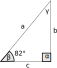
\includegraphics[width=0.3\textwidth]{trigo_06.pdf}
\end{figure}

L'incognita è $b$.

Gli elementi conosciuti sono:
\begin{itemize}
\item[$\beta$] = $82^{\circ}$
\item[$\alpha$] = $90^{\circ}$
\item[$c$] = $50$
\end{itemize}

L'angolo $\gamma$ è pari a $180-90-82=8^{\circ}$

Grazie al Teorema di Eulero (pagina \pageref{subs_euler}) sappiamo che 


\begin{equation*}
\frac{a}{\sin (\alpha)} = \frac{b}{\sin (\beta)} = \frac{c}{\sin (\gamma)}
\end{equation*}

quindi

\begin{equation*}
\frac{b}{\sin (82)} = \frac{50}{\sin (8)}
\end{equation*}

\begin{equation*}
b=\frac{50\cdot 0.990}{0.139}=356.115\textrm{ metri}
\end{equation*}

\vspace{1cm}
\hrule
\vspace{1cm}

\begin{minipage}{\textwidth}
Soluzione dell'esercizio \ref{etri_03} a pagina \pageref{etri_03}\label{stri_03}


\begin{equation*}
\frac{
\cos(x)
}{
\tan(x)\cdot\left(1-\sin(x)\right)
} = 1+\frac{1}{\sin(x)}
\end{equation*}


Per prima cosa moltiplico tutto per $\tan(x)$:

\begin{equation*}
\Rightarrow\frac{
\cos(x)
}{
\left(1-\sin(x)\right)
} = \tan(x)+\frac{\tan(x)}{\sin(x)}
\end{equation*}

Poi sostitsco $\tan(x)=\frac{\sin(x)}{\cos(x)}$:


\begin{equation*}
\Rightarrow\frac{
\cos(x)
}{
\left(1-\sin(x)\right)
} = \frac{\sin(x)}{\cos(x)}+\frac{1}{\cos(x)}
\end{equation*}

Porto $\frac{\sin(x)}{\cos(x)}$ a sinistra:

\begin{equation*}
\Rightarrow\frac{
\cos(x)
}{
\left(1-\sin(x)\right)
} 
-
\frac{\sin(x)}{\cos(x)}
= \frac{1}{\cos(x)}
\end{equation*}

Moltiplico $\frac{
\cos(x)
}{
\left(1-\sin(x)\right)
}$ per $\frac{\cos(x)}{\cos(x)}$ (che sarebbe $1$):

\begin{equation*}
\Rightarrow
\frac{\cos(x)}{\cos(x)}
\cdot
\frac{
\cos(x)
}{
\left(1-\sin(x)\right)
} 
-
\frac{\sin(x)}{\cos(x)}
= \frac{1}{\cos(x)}
\end{equation*}

\begin{equation*}
\Rightarrow
\frac{\cos^2(x)}{\cos(x)
\cdot
\left(1-\sin(x)\right)
} 
-
\frac{\sin(x)}{\cos(x)}
= \frac{1}{\cos(x)}
\end{equation*}

Moltiplico $\frac{\sin(x)}{\cos(x)}$ per $\frac{1-\sin(x)}{1-\sin(x)}$:

\begin{equation*}
\Rightarrow
\frac{\cos^2(x)}{\cos(x)
\cdot
\left(1-\sin(x)\right)
} 
-
\frac{\sin(x)}{\cos(x)}
\cdot
\frac{1-\sin(x)}{1-\sin(x)}
= \frac{1}{\cos(x)}
\end{equation*}

In questo modo i denominatori sono uguali quindi posso raccogliere:

\begin{equation*}
\Rightarrow
\frac{
\cos^2(x)-\sin(x)+\sin^2(x)}
{
\cos(x)\cdot
\left(1-\sin(x)\right)
} 
= \frac{1}{\cos(x)}
\end{equation*}

So che $\cos^2(x)+\sin^2(x)=1$:

\begin{equation*}
\Rightarrow
\frac{
1-\sin(x)
}{
\cos(x)\cdot
\left(1-\sin(x)\right)
} 
= \frac{1}{\cos(x)}
\end{equation*}

Semplifico togliendo $1-\sin(x)$:


\begin{equation*}
\Rightarrow
\frac{
1
}{
\cos(x)
} 
= \frac{1}{\cos(x)}
\end{equation*}

\end{minipage}
Soluzione dell'esercizio \ref{etri_04} a pagina \pageref{etri_04}\label{stri_04}

\begin{equation*}
\frac{
1+2\sin(x)\cos(x)
}{
\sin(x)+\cos(x)
}
=
\sin(x)+\cos(x)
\end{equation*}


\begin{equation*}
\Rightarrow
\frac{
1+2\sin(x)\cos(x)
}{
\sin(x)+\cos(x)
}
-(\sin(x)+\cos(x))
=
0
\end{equation*}

\begin{equation*}
\Rightarrow
\frac{
1+2\sin(x)\cos(x)
}{
\sin(x)+\cos(x)
}
-\frac{
\sin(x)+\cos(x)
}{
\sin(x)+\cos(x)
}\cdot(\sin(x)+\cos(x))
=
0
\end{equation*}


\begin{equation*}
\Rightarrow
\frac{
1+2\sin(x)\cos(x)
-(
\sin(x)+\cos(x)
)^2
}{
\sin(x)+\cos(x)
}
=
0
\end{equation*}


\begin{equation*}
\Rightarrow
\frac{
1+2\sin(x)\cos(x)
-(
\sin^2(x)+2\sin(x)\cos(x)+\cos^2(x)
)
}{
\sin(x)+\cos(x)
}
=
0
\end{equation*}


\begin{equation*}
\Rightarrow
\frac{
1+2\sin(x)\cos(x)
-\sin^2(x)-2\sin(x)\cos(x)-\cos^2(x)
}{
\sin(x)+\cos(x)
}
=
0
\end{equation*}


\begin{equation*}
\Rightarrow
\frac{
1+2\sin(x)\cos(x)-2\sin(x)\cos(x)-1
}{
\sin(x)+\cos(x)
}
=
0
\end{equation*}




\subsection{Soluzioni di esercizi nella sezione ``\textbf{\nameref{subsec:additional_log}}".}


Soluzione dell'esercizio \ref{exa_1} a pagina \pageref{exa_1}\label{sola_1}

\begin{equation*}
2\cdot \ln(6x - 2) = 5
\end{equation*}

\begin{equation*}
\ln(6x - 2) = \frac{5}{2}
\end{equation*}

\begin{equation*}
e^{\ln(6x - 2)} = e^{\frac{5}{2}}
\end{equation*}


\begin{equation*}
6x - 2 = e^{\frac{5}{2}}
\end{equation*}

\begin{equation*}
6x = 2+e^{\frac{5}{2}}
\end{equation*}


\begin{equation*}
x = \frac{2+e^{\frac{5}{2}}}{6}
\end{equation*}


\vspace{1cm}
\hrule
\vspace{1cm}

Soluzione dell'esercizio \ref{exa_2} a pagina \pageref{exa_2}\label{sola_2}

\begin{equation*}
e^{4x} - 3e^{2x} + 2 = 0
\end{equation*}


\begin{equation*}
\textrm{Poniamo }u=e^{2x}
\end{equation*}


\begin{equation*}
u^2-3u+2=0
\end{equation*}


\begin{equation*}
(u - 1)(u - 2) =0
\end{equation*}

\begin{equation*}
\left\{
\begin{array}{ll}
u=1 \\
u=2
\end{array}
\right.
\end{equation*}

\begin{equation*}
\left\{
\begin{array}{ll}
e^{2x}=1 \\
e^{2x}=2
\end{array}
\right.
\end{equation*}

\begin{equation*}
\left\{
\begin{array}{ll}
2x=\ln1 \\
2x=\ln2
\end{array}
\right.
\end{equation*}

\begin{equation*}
\left\{
\begin{array}{ll}
x=0 \\
x=\frac{\ln2}{2}
\end{array}
\right.
\end{equation*}



\vspace{1cm}
\hrule
\vspace{1cm}

Soluzione dell'esercizio \ref{exa_3} a pagina \pageref{exa_3}\label{sola_3}


\begin{equation*}
3^xe^{4x-1} = 5
\end{equation*}

\begin{equation*}
\ln ( 3^xe^{4x - 1} ) = \ln 5
\end{equation*}

\begin{equation*}
\ln 3^x + \ln ( e^{4x - 1} ) = \ln 5
\end{equation*}

\begin{equation*}
x\ln 3+4x-1=\ln 5
\end{equation*}

\begin{equation*}
x(\ln3 +4)=\ln 5 +1
\end{equation*}

\begin{equation*}
x=\frac{
1+\ln 5
}{
4+\ln 3
}
\end{equation*}

\vspace{1cm}
\hrule
\vspace{1cm}

\begin{minipage}{\textwidth}
Soluzione dell'esercizio \ref{exa_4} a pagina \pageref{exa_4}\label{sola_4}

La formula data è: 

\begin{equation*}
P = 1000 \cdot 1.0224t
\end{equation*}

Vogliamo $P=2000$, quindi 

\begin{equation*}
2000 = 1000 \cdot 1.022^{4t}
\end{equation*}

\begin{equation*}
2= 1.022^{4t}
\end{equation*}

Applichiamo il logaritmo da entrambe le parti:

\begin{equation*}
4t\cdot \lg 1.022 = \lg 2
\end{equation*}


\begin{equation*}
t=\frac{
\lg 2
}{
4\cdot\lg 1.022
} = 7.96
\end{equation*}

$\approx$ 8 years

\end{minipage}

\vspace{1cm}
\hrule
\vspace{1cm}


\subsection{Soluzioni di esercizi nella sezione ``\textbf{\nameref{subsec:calcolo_combinatorio}}".}

Soluzione dell'esercizio \ref{combl_01} a pagina \pageref{combl_01}\label{combs_01}

Ricordiamoci che 
\begin{equation*}
\binom{n}{k}=\frac{n!}{(n-k)!\cdot k!}
=\frac{
n\cdot(n-1)\times \cdots \times (n-k+1)
}{
k\cdot(k-1)\times \cdots \times 1
}
\end{equation*}

quindi

\begin{equation*}
\binom{n}{8}=\binom{n}{6}
\hspace{1cm}\Rightarrow \hspace{1cm}
\frac{n!}{(n-8)! \cdot 8!} = \frac{n!}{(n-6)! \cdot 6!}
\end{equation*}


\begin{equation*}
\frac{
\cancel{n} \cdot \cancel{(n-1)}\cdot(n-2) \cdots (n-7)\cdot \cancel{(n-8)}!
}
{
\cancel{(n-8)!} \cdot 8 \cdot 7 \cdot \cancel{6!}
} = \frac{
\cancel{n}\cdot\cancel{(n-1)}\cdots(n-5)\cancel{(n-6)!}
}{
\cancel{(n-6)!}\cdot\cancel{6!}
}
\end{equation*}

\begin{equation*}
(n-6)(n-7) = 56
\end{equation*}

$n=14; 14\ge 8 \Rightarrow $OK!

\vspace{1cm}
\hrule
\vspace{1cm}



Soluzione dell'esercizio \ref{combl_02} a pagina \pageref{combl_02}\label{combs_02}

\begin{equation*}
\frac{n\cdot(n-1)\cdot(n-2)\cdot
\cancel{(n-3)!}
}{
\cancel{(n-3)!}
} = 210
\end{equation*}

Viene un'equazione di $3^\circ$ grado ma

\begin{equation*}
210=7\cdot3\cdot2\cdot5
\end{equation*}

o meglio

\begin{equation*}
210=7\cdot6\cdot5
\end{equation*}

\begin{equation*}
210=7\cdot(7-1)\cdot(7-2)
\end{equation*}

quindi 

\begin{equation*}
n=7
\end{equation*}

\vspace{1cm}
\hrule
\vspace{1cm}



Soluzione dell'esercizio \ref{combl_03} a pagina \pageref{combl_03}\label{combs_03}

\begin{equation*}
\sum_{k=0}^{n}{\binom{n}{k}}=2^n
\end{equation*}

Ricordiamo la Binomial formula:

\begin{equation}
(x+y)^n=\sum_{k=0}^{n}{\binom{n}{k}x^{k}y^{n-k}}
=\sum_{k=0}^{n}{\binom{n}{k}x^{n-k}y^{k}}
\end{equation}

Si nota che è molto simile alla formulazione del problema.

Basterebbe trovare un $x$ e un $y$ tali per cui $x+y=2$, e la parte a sinistra diventerebbe proprio $2^n$.

Dopodiché basterebbe che questi $x$ e $y$ siano pari a $1$ quando elevati a potenza.

La soluzione è banale: scegliendo $x=1, y=1$ la \emph{Binomial formula} si riduce proprio alla formulazione del problema.

\vspace{1cm}

Un'altra dimostrazione fa uso della ricorsività.

Se si riesce a dimostrare che la formula è valida per un valore di partenza, e poi si dimostra che quando sia valida per un intero $k$ allora è valida anche per $k+1$, allora la dimostrazione è completa.

Come valore di base prendiamo $n=0$: la formula diventa 

\begin{equation*}
\sum_{k=0}^{0}{\binom{0}{k}}=\binom{0}{0}=\frac{0!}{0!\cdot0!}=2^0
\end{equation*}

perché ${0 \choose 0}$ è il numero di sottoinsiemi non ordinati di zero elementi che si possono ottenere da un insieme di zero elementi, quindi fa $1$.  $2^0$ a sua volta è pari a $1$.

Il primo passo è fatto; ora bisogna partire da un generico intero $k$ per il quale si suppone che la formula sia vera:

\begin{equation*}
\binom{k}{0} + \binom{k}{1} + \binom{k}{2} + \cdots + \binom{k}{k} = 2^k
\end{equation*}

E dimostrare che sia vera anche per $k+1$:


\begin{equation}\label{expr4}
\binom{k+1}{0} + \binom{k+1}{1} + \binom{k+1}{2} + \cdots + \binom{k+1}{k+1} = 2^{k+1}
\end{equation}

Ricordiamo la formula di Pascal (pagina \pageref{formula_pascal}), qui riscritta con il $k$ e $n$ invertiti per renderla più simile alla situazione in esame:


\begin{equation*}
{k \choose n}={k-1 \choose n}+{k-1 \choose n-1}
\end{equation*}

In base a questa formula ognuno degli addendi dell'espressione \ref{expr4} (tranne il primo) può essere riscritto come somma, per esempio


\begin{equation*}
{k+1 \choose 5}={k \choose 5}+{k \choose 4}
\end{equation*}

Questo non vale per il primo addendo perché si avrebbe un numero negativo nel binomio, quindi si lascia così com'è.

L'ultimo degli addendi a sua volta per il momento rimane invariato: ${k+1\choose k+1}$.

Quindi (a parte il primo e l'ultimo) ognuno degli addendi si ritrova doppio; prendiamone due per meglio illustrare la situazione:

\begin{equation*}
\cdots+{k+1\choose 6}+{k+1\choose 7}+\cdots
=
\cdots+{k\choose 6}+{k \choose 5}+{k\choose 7}+{k\choose 6}+\cdots
\end{equation*}

In questa ``fetta" della sommatoria ${k\choose 6}$ viene ripetuto due volte; questo vale anche per ${k\choose 5}$ che trova il suo doppione nell'addendo precedente, mentre ${k \choose 7}$ lo trova nel successivo.

Rivediamo ora il primo degli addendi e cioè ${k+1 \choose 0}$; esso vale $1$, come tutti i binomi con zero a denominatore.
Il secondo degli addendi dell'espressione \ref{expr4} e cioè ${k+1\choose 1}$ diventa ${k\choose 0}+{k\choose 1}$ e cioè $1+{k\choose 1}$.  Questo significa che anche il primo degli addendo trova il suo doppio.

L'ultimo degli addendi ${k+1\choose k+1}$ a sua volta vale 1, perché per definizione il numero di sottoinsiemi non ordinati di qualsiasi dimensione che sia uguale alla dimensione dell'insieme di partenza è sempre uno.  Quanti sottoinsiemi di un milione di elementi si possono definire partendo da un milione di elementi?  Uno.

Questo significa che ${k+1\choose k+1}={k\choose k}$.

Il penultimo degli addendi era ${k+1\choose k}$, che in base alla formiula di Pascal è diventato ${k\choose k}+{k\choose k-1}$.

Però ${k\choose k}$ a sua volta vale $1$, quindi anche l'ultimo addendo ha il suo doppione.  L'espressione \ref{expr4} è quindi diventata:

\begin{equation*}
{k\choose 0}+{k\choose 0}+
{k\choose 1}+{k\choose 1}+
{k\choose 2}+{k\choose 2}+\cdots+
{k\choose k-1}+{k\choose k-1}+
{k\choose k}+{k\choose k}
\end{equation*}

Che riscritto come sommatoria diventa:
\begin{equation*}
2\times\sum_{n=0}^k{{k\choose n}} = 2\times2^k=2^{k+1}
\end{equation*}

Entrambe le condizioni della dimostrazione ricorsiva sono soddisfatte, quindi il postulato è vero.



\subsection{Soluzioni di esercizi nella sezione ``\textbf{\nameref{sec:aritmetica}}".}

Soluzione dell'esercizio \ref{ari_01} a pagina \pageref{ari_01}\label{aris_01}

La risposta esatta è la ``B".

\[
2^{15} + 2^{15} = 2 \times 2^{15} = 2^{16}
\]


\vspace{1cm}
\hrule
\vspace{1cm}


Soluzione dell'esercizio \ref{ari_02} a pagina \pageref{ari_02}\label{aris_02}

La risposta esatta è la ``A".

I numeri $100$ e $440$ non sono primi perché pari (divisibili per $2$).


Il numero $231$ non è primo perché è divisibile per $3$, in base al criterio di divisibilità per
3: ``se la somma delle cifre di un numero è divisibile per 3, il numero è divisibile per 3".  In questo 
caso $2 + 3 + 1 = 6$ che è divisibile per 3.

Il numero $91$ è primo?
In generale per decidere se un numero $n$ è primo occorre verificare che non sia divisibile per nessun numero 
primo compreso tra 2 e $\sqrt{n}$.

Inoltre, per i criteri di divisibilità, $91$ non è divisibile per $2$ né per $3$ o per $5$.
È è divisibile per $7$?
Sì, perché
\[
 91 = 70 + 21 = 7 \times 10 + 7 \times 3 = 7 \times 13
\]

Il numero $1003$ è primo? I criteri di divisibilità dicono che non è divisibile per $2$, $3$, $5$, $11$.
Per essere certi che sia primo, dobbiamo verificare che non sia divisibile per nessun numero
primo $\leq \sqrt{1003}$, ossia (oltre a quelli già elencati), per
\[
7, 13, 17, 19, 23, 29, 31
\]

Carta, penna e pazienza ci dicono che
\begin{itemize}
\item $\frac{1003}{7}= 143$ con resto $2$
\item $\frac{1003}{13} = 77$ con resto $2$
\item $\frac{1003}{17} = 59$ con resto $0$
\end{itemize}

Dunque 
\[
1003 = 17 \times 59
\]

Nemmeno $1003$ è primo. 





\subsection{Soluzioni di esercizi nella sezione ``\textbf{\nameref{subsec:limiti:successioni}}".}

Soluzione dell'esercizio \ref{lims_00} a pagina \pageref{lims_00}\label{limss_00}

In base alla definizione bisogna dimostrare che per un qualsiasi$\varepsilon > 0$
vale questa disuguaglianza: 

\[
\left|
\frac{
n
}{
2n+5
}-\frac{1}{2}
\right|
<\varepsilon
\]


\[
\left|
\frac{
2n -2n -5
}{
4n+10
}
\right|
<\varepsilon
\]


\[
\left|
\frac{
-5
}{
4n+10
}
\right|
<\varepsilon
\]

Si può togliere il modulo (valore assoluto) perché i due termini della disuguaglianza sono entrambi positivi:


\[
\frac{
-5
}{
4n+10
}
<\varepsilon
\]


\[
5
<\varepsilon
\cdot(4n+10)
\]



\[
5
<4n\varepsilon+10\varepsilon
\]

Ora si risolve per $n$

\[
-4n\varepsilon
<
-5
+10\varepsilon
\]


\[
-n
<
\frac{
-5
+10\varepsilon
}{4\varepsilon}
\]

ossia 

\[
n
>
\frac{
5
-10\varepsilon
}{4\varepsilon}
\]

Questo significa che per qualsiasi $\varepsilon$ è possibile calcolare un numero $n$ che soddisfa la definizione, quindi la dimostrazione è fatta.

\vspace{1cm}
\hrule
\vspace{1cm}



Soluzione dell'esercizio \ref{lims_01} a pagina \pageref{lims_01}\label{limss_01}

Come sempre in questo tipo di esercizi, bisogna dimostrare che dato un $\varepsilon > 0$, esiste un $n_0$ tale per cui
\[
\forall n>n_0: \left| a_n - a \right| < \varepsilon
\]

Nel caso dell'esercizio:
\[
a_n = \frac{n-1}{n} \textrm{\hspace{1cm}mentre \hspace{1cm}} a=1
\]

quindi la disequazione diventa:

\[
\left| \frac{n-1}{n} -1 \right| < \varepsilon
\]

ossia

\[
\left| \frac{n-1-n}{n} \right| < \varepsilon
\]

\[
\left| \frac{1}{n} \right| < \varepsilon
\]

Siccome $\frac{1}{n}$ è una quantità positiva, possiamo tralasciare il valore assoluto:


\[
\frac{1}{n} < \varepsilon \hspace{1cm} \Rightarrow  \hspace{1cm} n > \frac{1}{\varepsilon}
\]

Concludendo, per qualsiasi $\varepsilon$ è possibile calcolare un numero $n$ tale per cui la definizione di limite è vera, quindi il limite della successione è effettivamente pari a $1$.



\vspace{1cm}
\hrule
\vspace{1cm}



Soluzione dell'esercizio \ref{lims_02} a pagina \pageref{lims_02}\label{limss_02}

\[
\lim_{n \to +\infty}\frac{2n+1}{3n-1}=
\]

Raccogliere $n$

\[
\lim_{n \to +\infty}\frac{n
\left( 
	2+\frac{1}{n}
\right)
}{n
\left( 
	3-\frac{1}{n}
\right)
}=
\]

Semplificare

\[
\lim_{n \to +\infty}\frac{
	2+\frac{1}{n}
}{
	3-\frac{1}{n}
}=
\]

Per $n$ che tende all'infinito $\frac{1}{n}$ tende a zero, quindi


\[
\lim_{n \to +\infty}\frac{
	2+\frac{1}{n}
}{
	3-\frac{1}{n}
}=\frac{2}{3}
\]

Ora come al solito bisogna usare la definizione di limite per dimostrare che 

\[
\lim_{n \to +\infty}\frac{2n+1}{3n-1}=\frac{2}{3}
\]

quindi dato un $\varepsilon > 0$ trovare un $n_0$ tale che per ogni $n>n_0$ si abbia
% https://www.youmath.it/forum/tutto-sulle-funzioni-da-r-a-r-e-sui-numeri-reali-analisi-matematica/39870-verificare-il-limite-di-una-successione-fratta-con-la-definizione.html

\[
\left|
\frac{2n+1}{3n-1}-\frac{2}{3}
\right| < \varepsilon
\]

\[
\left|
\frac{
3(2n+1)-2(3n-1)
}{
(3n-1)3
}
\right| < \varepsilon
\]

\[
\left|
\frac{
\cancel{6n}+3-\cancel{6n}+2
}{
9n-3
}
\right| < \varepsilon
\]

\[
\left|
\frac{
5
}{9n-3}
\right| < \varepsilon
\]

Entrambi i tyermini sono positivi quindi non serve il valore assoluto:

\[
\frac{
5
}{9n-3}
< \varepsilon
\]

Ora bisogna risolvere per $n$:

\[
\frac{
5
}{9n-3}
- \varepsilon <0
\]


\[
\frac{5 -9n\varepsilon +3\varepsilon
}{9n-3
} < 0
\]

Il denominatore ($9n-3$) è sempre positivo perché per definizione $n$ è positivo.

Quindi la disequazione si riduce a:

\[
5-9n\varepsilon +3\varepsilon < 0
\]

\[
-9n\varepsilon < -5 -3\varepsilon
\]

\[
n > \frac{5+3\varepsilon}{9\varepsilon}
\]

Dato un qualsiasi $\varepsilon$ esiste quindi un numero $n_0 = \frac{5+3\varepsilon}{9\varepsilon}$ tale per cui qualsiasi $n>n_0$ soddisfa la definizione di limite: la dimostrazione è terminata.


\subsection{Soluzioni di esercizi nella sezione ``\textbf{\nameref{subsec:the:circle}}"}

% https://math.libretexts.org/Courses/Monroe_Community_College/MTH_165_College_Algebra_MTH_175_Precalculus/03%3A_Polynomial_and_Rational_Functions/3.02%3A_Circles/3.2e%3A_Circle_Exercises.
% https://math.libretexts.org/Courses/Monroe_Community_College/MTH_165_College_Algebra_MTH_175_Precalculus/03%3A_Polynomial_and_Rational_Functions/3.02%3A_Circles/3.2e%3A_Circle_Exercises.

Soluzione dell'esercizio \ref{circ_00} a pagina \pageref{circ_00}\label{circs_00}

\[
(x-8)^2+(y+10)^2=64
\]

\vspace{1cm}
\hrule
\vspace{1cm}


Soluzione dell'esercizio \ref{circ_01} a pagina \pageref{circ_01}\label{circs_01}

Center: $(2,1)$

Radius: $r=2$
\[
(x-2)^2+(y+1)^2=4
\]

\vspace{1cm}
\hrule
\vspace{1cm}


Soluzione dell'esercizio \ref{circ_02} a pagina \pageref{circ_02}\label{circs_02}

Center: $(-1,3)$

Radius:  $r=5$

\[
(x+1)^2+(y-3)^2=25  
\]

\vspace{1cm}
\hrule
\vspace{1cm}


Soluzione dell'esercizio \ref{circ_03} a pagina \pageref{circ_03}\label{circs_03}

\begin{itemize}
\item[a] Center $(2,-3)$, radius  $r=3$
\item[b] Center $(2,-5)$, radius  $r=2$
\item[c] Center $(-9,0)$, radius  $r=5$
\item[d] Center $(-\frac{1}{2},\frac{3}{5})$, radius  $r=\frac{\sqrt{161}}{10}$
\end{itemize}


\begin{figure}[H]
\centering
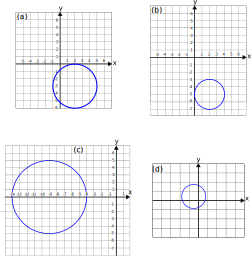
\includegraphics[width=0.9\textwidth]{circles_02.pdf}
\end{figure}




\vspace{1cm}
\hrule
\vspace{1cm}


Soluzione dell'esercizio \ref{circ_04} a pagina \pageref{circ_04}\label{circs_04}

\vspace{1cm}

Bisogna riscrivere l'equazione 

\[
x^2+y^2-6x+8y+24=0 
\]

nella forma dell'equazione standard del cerhio (l'equazione \ref{cerchio:equazione} a pagina \pageref{cerchio:equazione}):


\[
(x-h)^2+(y-k)^2=r^2
\]

Per fare ciò, spostiamo i termini variabili alla sinistra e le costanti a destra del segno di uguaglianza, e concentriamo l'attenzione sui termini con la $x$:

\begin{equation} \label{circ:04:1}
\underline{x^2-6x}+y^2+8y=-24
\end{equation}

Ora teniamo bene a mente come è fatto il quadrato del binomio:

\[
(x-h)^2 = x^2-2hx +h^2
\]

Guardando bene i termini con la $x$ nell'espressione \ref{circ:04:1}, troveremo che quel $-6x$ somiglia molto a $2\times -3\times x$, quindi basterebbe avere un $9$ per poter costruire un perfettamente plausibile quadrato: $x^2-6x+9$, il che ci direbbe che $h=-3$.

Possiamo aggiungere $9$ ad entrambi i termini dell'uguaglianza:


\[
\underline{x^2
-6x
+9
}
+y^2
+8y=-24 + 9 
\]

Ora possiamo raggruppare $x$:


\[
\underline{(x-3)^2 }
+y^2
+8y=-24 + 9 
\]

Facciamo lo stesso giochino con le $y$ , in quanto $+8y$ è $2\times 4 \times y$ quindi aggiungiamo $16$ da entrambe le parti come abbiamo fatto prima:

\[
(x-3)^2 
+y^2
+8y
+16
=-24 + 9 +16
\]

Ora l'equazione diventa:

\[
(x-3)^2+ 
(x+4)^2
=1
\]


Abbiamo quindi trovato i valori che ci serviuvano e cioè $h=3$, $k=-4$, $r=1$.

In altre parole il nostro cerchio ha il centro in $(3,-4)$ e un raggio pari a $1$.



\vspace{1cm}
\hrule
\vspace{1cm}


Soluzione dell'esercizio \ref{geop_01} a pagina \pageref{geop_01}\label{geos_01}

The tangent(s) are of the form $y = mx + 14$ because they go through $(0,14)$.

Substitute this into the equation of the circle:


\[
x^2+y^2+14x-6y=-41
\]

\[
x^2+(mx+14)^2+14x-6(mx+14)+41=0
\]


\[
x^2+m^2x^2+28mx+196+14x-6mx-43=0
\]

\[
(1+m^2)x^2+(22m+14)x+153=0
\]

This is a quadratic equation: $ax^2+bx+c=0$
where
\begin{enumerate}
\item $a=1+m^2$
\item $b=22m+14$
\item $c=153$
\end{enumerate}

The discriminant ($b^2-4ac$) tells us how many solutions does the equation have.

In this case we are looking for a single solution because the lines are tangent to the circle, i.e. each line touches the circle in one point only.

So the discriminant (often written as $\Delta$) must be zero:

\[
(22m+14)^2-4(1+m^2)153=0
\]

\[
484m^2+616m+196-612-612m^2=0
\]

\[
-128m^2+616m-416=0
\]

Now this is a simple quadratic equation, let's apply the formula:

\[
m=\frac{-b\pm\sqrt{b^2-4ac}}{2a}=\frac{-616\pm \sqrt{616^2-4\times(-128)\times(-416)}}{2\times -128}
\]


\[
m=\frac{-616\pm \sqrt{379456-212992}}{-256}
\]


\[
m=\frac{-616\pm 408}{-256}
\]

\[
\left\{
\begin{array}{ll}
m_1=\frac{-616+408}{-256}=\frac{-208}{-256}=\frac{13}{16}\\
\\
m_2=\frac{-616-408}{-256}=4
\end{array}
\right.
\]

\[
\left\{
\begin{array}{ll}
l_1: y=\frac{13}{16}x+14\\
\\
l_2: y=4x+14
\end{array}
\right.
\]

\vspace{1cm}
\hrule
\vspace{1cm}


Soluzione dell'esercizio \ref{circ_06} a pagina \pageref{circ_06}\label{circs_06}

È necessario per prima cosa riscrivere le equazioni nella seguente forma:

\[
(x-h)^2+(y-k)^=r^2
\]

dove 
\begin{itemize}
\item[\textbf{h}] è la coordinata $x$ del centro
\item[\textbf{k}] è la coordinata $y$ del centro
\item[\textbf{r}] è il raggio
\end{itemize}

Raccogliendo per $x$ e $y$ otteniamo: 

\[
\begin{split}
(a): (x^2-2x)+(y^2-4y)=4 \\
\\
(b): (x^2-4x)+(y^2-2y)=-4
\end{split}
\]

Facendo riferimento per ora alla sola equazione $(a)$, per trasformare
i termini $(x^2-2x)$ e $(y^2-4y)$ nella forma $(x-h)^2, (y-k)^2$ dobbiamo
seguire per ognuno dei termini questi passi:

\begin{enumerate}
\item considerare il coefficiente del termine di primo grado
\item dividere per $2$
\item calcolarne il quadrato
\item aggiungere il risultato da entrambi i lati dell'equazione
\end{enumerate}

Questo significa che per il termine $(x^2-2x)$ avremo:

\begin{enumerate}
\item il coefficiente del termine di primo grado è $2$
\item $2/2=1$
\item $1^2=1$
\item aggiungere questo risultato a entrambi i lati dell'equazione, che diventa:
\[
(a): (x^2-2x+1)+(y^2-4y)=4+1
\]
\end{enumerate}

Per il termine $(y^2-4y)$ avremo che:
\begin{enumerate}
\item il coefficiente del termine di primo grado è $4$
\item $4/2=2$
\item $2^2=4$
\item aggiungere il risultato a entrambi i lati dell'equazione, che diventa:
\[
(a): (x^2-2x+1)+(y^2-4y+4)=4+1+4
\]
\end{enumerate}

A questo punto possiamo riscrivere l'equazione come segue:

\[
(a) (x-1)^2+(y-2)^2=3^2
\]

Quindi la prima circonferenza avrà il centro in $(1, 2)$ e raggio 3.

Allo stesso modo la seconda equazione potrà essere riscritta come segue:
\[
(b) (x-2)^2+(y-1)^2=1
\]

Quindi la seconda circonferenza avrà il centro in $(2, 1)$ e raggio 1.

Un veloce grafico ci dirà che la soluzione esatta è la $B$:
le due circonferenze sono disgiunte e la seconda è interna alla prima.

\begin{figure}[H]
\centering
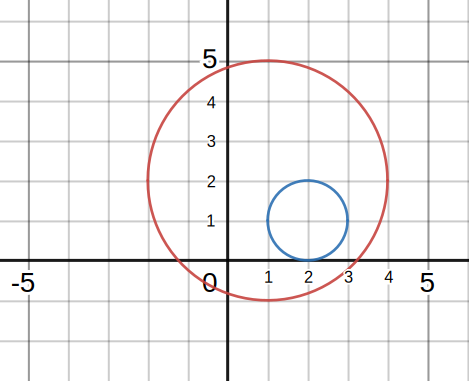
\includegraphics[width=0.6\textwidth]{circ_06.pdf}
\end{figure}

N.B.: la risposta $D$ era comunque da scartare in quanto due circonferenze
possono avere solo zero punti in comune (disgiunte) oppure un
punto in comune (tangenti) oppure due punti in comune (intersecanti),
oppure infiniti punti in comune (identiche e sovrapposte).



%\vspace{1cm}
%\hrule
%\vspace{1cm}
%
%
%Soluzione dell'esercizio \ref{circ_07} a pagina \pageref{circ_07}\label{circs_07}
%
%\vspace{1cm}
%\hrule
%\vspace{1cm}
%
%
%Soluzione dell'esercizio \ref{circ_08} a pagina \pageref{circ_08}\label{circs_08}
%
%\vspace{1cm}
%\hrule
%\vspace{1cm}
%
%
%Soluzione dell'esercizio \ref{circ_09} a pagina \pageref{circ_09}\label{circs_09}
%
%\vspace{1cm}
%\hrule
%\vspace{1cm}
%
%
%Soluzione dell'esercizio \ref{circ_10} a pagina \pageref{circ_10}\label{circs_10}
%
%\vspace{1cm}
%\hrule
%\vspace{1cm}
%




\subsection{Soluzioni di esercizi nella sezione ``\textbf{\nameref{sec:funzioni}}"}

Soluzione dell'esercizio \ref{exf_1} a pagina \pageref{exf_1}\label{solf_1}

\[
x^2 - 6x + k > 2
\]

Trasformiamo i termini $x^2-6x$ nel quadrato di un binomio e cioè nella forma $(ax+b)^2$.

Il valore di $a$ è pari a $1$; il valore di $b$ sarà tale per cui $2ab=-6$, quindi $2b=-6$, cioè $b=-3$.

\[ (x-3)^2=x^2-6x+9 \]

L'espressione da inserire al posto di $x^2 - 6x$ è $(x-3)^2 -9$:

\[ (x-3)^2-9+k>2 \]

\[ k>11-(x-3)^2 \]

$(x-3)^2$ non può che essere positivo, quindi il suo massimo valore è zero:

\[k>11\]


\vspace{1cm}
\hrule
\vspace{1cm}






\end{document}

